\documentclass[11pt,a4paper]{article}

\usepackage[margin=24mm,headheight=15pt]{geometry}
\usepackage[T1]{fontenc}
\usepackage[utf8]{inputenc}
\usepackage{lmodern}
\usepackage{microtype}
\usepackage{amsmath,amssymb,mathtools,bm}
\usepackage{booktabs,tabularx,longtable,array,multirow}
\usepackage{graphicx}
\usepackage{subcaption}
\usepackage{xcolor}
\usepackage{enumitem}
\usepackage{fancyhdr}
\usepackage{hyperref}
\usepackage{url}
\usepackage{float}
\usepackage{listings}
\usepackage{caption}

\definecolor{navy}{HTML}{16324F}
\definecolor{blue}{HTML}{2F6690}
\definecolor{lightblue}{HTML}{EAF2F8}
\definecolor{darkgray}{HTML}{3C4858}
\definecolor{lightgray}{HTML}{F3F5F7}
\definecolor{red}{HTML}{A23B3B}
\hypersetup{
  colorlinks=true,
  linkcolor=navy,
  citecolor=blue,
  urlcolor=blue,
  pdftitle={Time-varying Minimum-Variance Portfolios and Dynamic CVaR Extensions},
  pdfauthor={Independent reproduction and extension project}
}
\urlstyle{same}
\graphicspath{{../results/plots/}{results/plots/}}
\captionsetup{font=small,labelfont=bf}
\setlist{nosep,leftmargin=1.6em}
\setlength{\parindent}{0pt}
\setlength{\parskip}{0.55em}
\setlength{\emergencystretch}{2em}
\renewcommand{\arraystretch}{1.13}
\allowdisplaybreaks
\raggedbottom
\newcolumntype{Y}{>{\raggedright\arraybackslash}X}
\newcolumntype{L}[1]{>{\raggedright\arraybackslash}p{#1}}

\pagestyle{fancy}
\fancyhf{}
\lhead{TV-MVP reproduction and extensions}
\rhead{Technical report}
\cfoot{\thepage}

\newcommand{\R}{\mathbb{R}}
\newcommand{\E}{\mathbb{E}}
\newcommand{\Var}{\operatorname{Var}}
\newcommand{\Cov}{\operatorname{Cov}}
\newcommand{\VaR}{\operatorname{VaR}}
\newcommand{\ES}{\operatorname{ES}}
\newcommand{\CVaR}{\operatorname{CVaR}}
\newcommand{\one}{\bm{1}}
\newcommand{\wh}{\widehat}
\newcommand{\trans}{^{\mathsf T}}
\newcommand{\code}[1]{\texttt{#1}}
\newcommand{\pct}[1]{#1\%}
\newcommand{\noteBox}[1]{%
  \begin{center}\colorbox{lightblue}{\parbox{0.93\linewidth}{\textbf{Interpretation note.} #1}}\end{center}}
\newcommand{\warningBox}[1]{%
  \begin{center}\colorbox{lightgray}{\parbox{0.93\linewidth}{\textbf{Important limitation.} #1}}\end{center}}

\lstset{
  basicstyle=\ttfamily\small,
  backgroundcolor=\color{lightgray},
  frame=single,
  rulecolor=\color{lightgray},
  breaklines=true,
  columns=fullflexible,
  keepspaces=true,
  showstringspaces=false
}

\title{\vspace{-1.2cm}\textbf{Time-varying Minimum-Variance Portfolios\\and Dynamic CVaR Extensions}\\[0.5em]
\large A complete mathematical, computational, empirical, and statistical account}
\author{Independent reproduction-and-extension project}
\date{6 September 2026}

\begin{document}
\maketitle

\begin{abstract}
This report explains the entire repository as a self-contained research project. It first reconstructs the mathematical and computational logic of Fan, Wu, Yang, and Zhong's time-varying minimum-variance portfolio (TV-MVP), using the authors' public manual and unchanged MATLAB/R release. It then documents the portable Python reproduction, a dynamic factor-covariance extension, empirical factor-bootstrap CVaR, a constraint-matched comparison, and a filtered, stressed, regularised CVaR repair. Every estimation date uses only trailing information. The empirical study uses 39 long-history stocks selected from a current NIFTY 50 list, a 504-trading-day window, and monthly rebalancing. Statistical uncertainty is evaluated with paired moving-block bootstrap intervals on monthly losses; regimes, covariance forecasts, factor diagnostics, tail calibration, simulations, and parameter sensitivity are also studied. The principal empirical conclusion is deliberately limited: raw empirical CVaR is poorly calibrated and unstable after 2021; filtered scenarios and regularisation materially improve its point estimates, but do not establish statistically reliable superiority over a constraint-matched MVP. Equal weight has the highest realised return and Sharpe ratio in this sample. The project is a rigorous exploratory extension, not evidence of future profitability.
\end{abstract}

\noteBox{The words ``original'', ``benchmark'', and ``author-style'' refer to the public methodology and code release. The journal paper's original proprietary empirical dataset is not in the repository. Consequently, the project reproduces the public simulation/example workflow as closely as portable software allows; it does not claim an exact replication of every journal table.}

\tableofcontents
\listoftables
\listoffigures
\clearpage

\section{Executive overview}

\subsection{The scientific question}

For a portfolio of $p$ assets, the minimum-variance problem depends on the conditional return covariance matrix. A conventional sample covariance assumes that the joint distribution is sufficiently stable inside the estimation window. Fan et al.\ relax that assumption by allowing factor loadings to vary smoothly over time while keeping factor and residual covariance components constant over the local estimation period \cite{fan2024}. Their estimator is
\begin{equation}
  \wh\Sigma_{r,t}^{\text{{TV}}}
  = \wh B_t\wh\Sigma_F\wh B_t\trans + \wh\Sigma_e.
  \label{eq:base-cov}
\end{equation}
The first repository extension lets factor risk itself change:
\begin{equation}
  \wh\Sigma_{r,t}^{\text{{dyn}}}
  = \wh B_t\wh\Sigma_{F,t}^{\text{{EWMA}}}\wh B_t\trans + \wh\Sigma_e.
  \label{eq:dynamic-cov}
\end{equation}
The second extension stops treating variance as the only risk criterion. It creates return scenarios from the fitted local factor model and chooses weights to minimise 95\% loss CVaR. A final follow-up addresses observed scenario-tail miscalibration with filtered historical simulation, recency weighting, explicit stress draws, and $L_1$ portfolio regularisation.

\subsection{The strategies}

The repository uses the following labels.

\begin{table}[H]
\centering
\caption{Strategy definitions}
\label{tab:strategies}
\small
\begin{tabularx}{\textwidth}{@{}L{0.20\textwidth}YL{0.25\textwidth}@{}}
\toprule
Label & Construction & Default feasible set \\
\midrule
A: Equal weight & $w_i=1/p$ at each rebalance & Long only; no active cap issue because $1/39<10\%$ \\
B: Original TV-MVP & Equation \eqref{eq:base-cov}, then minimum variance & Unconstrained in the core run \\
C: Dynamic-$\Sigma_F$ TV-MVP & Equation \eqref{eq:dynamic-cov}, then minimum variance & Unconstrained in the core run \\
D: Empirical CVaR & Paired block-bootstrap factor/residual scenarios & Long only; 10\% maximum weight \\
D-FS: Filtered/stressed CVaR & Current-state rescaling, recent blocks, stress mixture & Long only; 10\% cap \\
D-REG: Regularised filtered CVaR & D-FS plus turnover and diversification penalties & Long only; 10\% cap \\
\bottomrule
\end{tabularx}
\end{table}

The core A--D comparison intentionally preserves the requested original unconstrained MVP benchmark, but it is not a pure objective comparison because D has a different feasible set. The later matched experiment gives B, C, and all CVaR variants identical long-only, 10\%-cap constraints. Results from the matched experiment are the appropriate answer to ``MVP versus CVaR under the same portfolio rules.''

\subsection{Main numerical findings}

Across the full February 2017--August 2026 out-of-sample period, equal weight has the highest annualised return and Sharpe ratio. Dynamic factor covariance is extremely close to the original covariance estimator. Raw empirical CVaR has slightly lower full-sample daily volatility and ES than the unconstrained benchmark, but lower return and deeper drawdown.

After 2021, the fair matched comparison reverses the apparent tail-risk advantage: empirical CVaR has higher realised volatility, ES, drawdown, and turnover than both matched MVPs. Its fitted scenario CVaR is lower, but subsequent realised tail loss is higher. This is evidence of scenario-tail estimation error, not a linear-programming failure.

The pre-specified repair raises empirical CVaR's post-2021 annualised net return from 10.17\% to 14.30\% and lowers annual turnover from 4.75 to 3.50. Its fitted-versus-realised daily CVaR gap falls from 0.219 percentage point to 0.005 percentage point. Nevertheless, its paired monthly differences from matched original MVP all have 95\% bootstrap intervals containing zero. The correct conclusion is ``promising exploratory repair'', not ``superior strategy.''

\section{Repository provenance, organisation, and research scope}

\subsection{What was supplied}

The initial repository was an author code release comprising 26 files: a 16-page user manual, MATLAB functions, one R bridge script, a Windows batch file, two MATLAB data files, and an example CSV. Every supplied file was moved without content changes into \path{original_author_code/}. Byte-level SHA-256 comparisons against Git history were performed for all 26 files after reorganisation.

The author workflow assumes MATLAB, CVX, Windows \code{dos}, and R packages \code{spcov}, \code{PDSCE}, and \code{R.matlab}. The extension is implemented in Python because that dependency chain is not portable in the present environment. The Python implementation is not passed off as the literal author executable.

\subsection{Independent project structure}

\begin{table}[H]
\centering
\caption{Top-level project organisation}
\label{tab:layout}
\begin{tabularx}{\textwidth}{@{}lX@{}}
\toprule
Path & Purpose \\
\midrule
\path{original_author_code/} & Untouched author MATLAB/R release and manual \\
\path{src/tvmvp_ext/} & Portable estimation, optimisation, backtesting, inference, diagnostics, and simulation library \\
\path{scripts/} & Reproduction, empirical, diagnostic, matched, improved-CVaR, simulation, and all-in-one entry points \\
\path{data/raw/} & Frozen adjusted-close and NIFTY index snapshots \\
\path{results/tables/} & Machine-readable numerical evidence \\
\path{results/plots/} & Saved diagnostics and performance figures \\
\path{tests/} & Constraint, timing, covariance, bootstrap, and reproducibility tests \\
\path{config.yaml} & Single source of model and evaluation parameters \\
\path{01_...md}--\path{06_...md} & Concise staged reports and follow-up investigations \\
\path{report/} & This complete LaTeX source \\
\bottomrule
\end{tabularx}
\end{table}

\subsection{Claims that are and are not in scope}

The project can support claims about the behaviour of these implementations on the frozen sample and stated DGPs. It cannot establish that any portfolio will outperform in the future, that results survive point-in-time universe construction, or that the portable sparse estimator is numerically identical to the author R estimator. The improved CVaR specification was fixed in \path{config.yaml} before its one reported run, but it was designed after observing the earlier NIFTY failure. It is therefore internally pre-specified for the follow-up comparison but not an externally registered, fully independent confirmatory test.

\section{Data, timing, and information sets}

\subsection{Author example data}

The supplied \path{example_data.mat} contains a $50\times500$ return matrix named \code{R0}. The manual's example uses observations 1--250 for the first estimate, holds for five days, and repeats weekly through observation 500. It reports daily Sharpe-like ratios, means, and standard deviations for TV-MVP and $1/N$.

The synthetic author DGP uses $p=50$, $T=200$ or 250, two AR(1) factors, smooth stochastic loadings, and Toeplitz residual covariance $(\Sigma_e)_{ij}=0.5^{|i-j|}$. Section \ref{sec:reproduction} gives the exact equations and reproduction outcome.

\subsection{NIFTY empirical snapshot}

The extension requested adjusted-close returns beginning in 2015. The frozen data manifest records:

\begin{itemize}
  \item source: Yahoo Finance adjusted-close field retrieved through \code{yfinance};
  \item requested dates: 1 January 2015 through 5 September 2026, with the end date exclusive at download;
  \item observed prices: 1 January 2015 through 4 September 2026;
  \item requested universe: 40 names drawn from a current NIFTY 50 constituent list;
  \item retained universe: 39 names; \code{TRENT.NS} returned no usable history;
  \item minimum completeness rule: 98.5\%; all retained series were recorded as complete before limited filling;
  \item frozen stock-file SHA-256: \code{e6d40f9f3eba...8a55};
  \item frozen index-file SHA-256: \code{b0f0307ea507...571e}.
\end{itemize}

Adjusted-close simple returns are
\begin{equation}
 r_{i,t}=\frac{P^{\text{adj}}_{i,t}}{P^{\text{adj}}_{i,t-1}}-1.
\end{equation}
Prices and the NIFTY index are aligned on common dates. At most three consecutive missing prices are forward-filled, then any row with a remaining stock missing is removed. Returns are not converted to excess returns because no daily risk-free series is present. Consequently, ``Sharpe ratio'' in this project is mean return divided by standard deviation with a zero risk-free rate, not the exact excess-return Sharpe ratio used in some finance studies.

\warningBox{The stock universe is selected using current constituents and long histories. Delisted firms and past constituents that later left the index are absent. This creates survivorship and lookback-selection bias even though the rolling estimators themselves do not use future returns. A publishable confirmatory study should use point-in-time membership and delisting returns.}

\subsection{Rolling chronology and no-look-ahead rule}

Let $d_j$ be the last trading date of month $j$. With window length $W=504$, the estimator at $d_j$ receives only
\begin{equation}
 \mathcal I_{d_j}=\{r_{d_j-W+1},\ldots,r_{d_j}\}.
\end{equation}
Weights are computed after $d_j$ and take effect on the next trading date. They remain in force, with natural within-period drift, through $d_{j+1}$. No return dated after $d_j$ enters estimation or scenario generation for that rebalance. A dedicated test perturbs the last ten observations and verifies that all earlier weights remain identical.

The out-of-sample sample contains 2,362 trading days, from 1 February 2017 through 31 August 2026, generated by 115 rebalance decisions dated 31 January 2017 through 31 July 2026. September 2026 is excluded because a complete next monthly holding interval was not available.

\section{Base-paper mathematical framework}
\label{sec:base-math}

\subsection{Locally time-varying factor model}

Let $r_t=(r_{1t},\ldots,r_{pt})\trans\in\R^p$ denote returns and $f_t\in\R^K$ latent common factors. The base model is
\begin{equation}
 r_t=B_t f_t+e_t,
 \qquad B_t=B(t/T),
 \label{eq:factor-model}
\end{equation}
where $B(\cdot)$ changes smoothly in rescaled time, while $e_t$ contains idiosyncratic returns. A convenient identification is $T^{-1}\sum_t f_tf_t\trans=I_K$, with factor rotations otherwise observationally equivalent. Under contemporaneous factor-residual orthogonality,
\begin{equation}
 \Sigma_{r,t}=\Cov(r_t\mid\mathcal I_{t-1})
 =B_t\Sigma_F B_t\trans+\Sigma_e.
 \label{eq:population-factor-cov}
\end{equation}
The authors' key modelling choice is that time variation in $\Sigma_{r,t}$ is transmitted primarily through $B_t$, whereas $\Sigma_F$ and $\Sigma_e$ are estimated over the window as constant. This is more flexible than a constant-loading factor model, but less flexible than a fully time-varying covariance decomposition.

\subsection{Boundary-adjusted Epanechnikov weighting}

For target date $r$ and observation $t$, define $u_{tr}=(t-r)/(Th)$. The interior Epanechnikov kernel is
\begin{equation}
 K(u)=\frac34(1-u^2)\mathbf 1(|u|\le1).
\end{equation}
The author \code{Kernel2.m} divides the kernel by its truncated integral near the left and right sample boundaries, following the boundary-correction idea cited to Hong and Li and Su and Wang \cite{hongli2005,suwang2017}. In schematic form,
\begin{equation}
 K^*_{r}(u)=
 \begin{cases}
 K(u)\big/\int_{-r/(Th)}^1K(v)\,dv,&r<Th,\\
 K(u),&Th\le r\le T-Th,\\
 K(u)\big/\int_{-1}^{(1-r/T)/h}K(v)\,dv,&r>T-Th.
 \end{cases}
\end{equation}
The MATLAB weight is $k^*_{h,tr}=h^{-1}K_r^*(u_{tr})$. The Python port uses the same compact-support kernel but normalises the discrete weights to sum to one. Because factor scores and loadings can be reciprocally rescaled, the resulting common covariance is the meaningful object for comparison.

The rule-of-thumb bandwidth is
\begin{equation}
 h=\frac{2.35}{\sqrt{12}}T^{-1/5}p^{-1/10}.
 \label{eq:bandwidth}
\end{equation}

\subsection{Local principal components}

Store returns as $R=[r_1,\ldots,r_T]\in\R^{p\times T}$. At target $r$, form the weighted data matrix
\begin{equation}
 X_r=D_rR\trans,
 \qquad D_r=\operatorname{diag}\big(\sqrt{k^*_{h,1r}},\ldots,\sqrt{k^*_{h,Tr}}\big).
\end{equation}
Local PCA solves the rank-$K$ approximation problem
\begin{equation}
 \min_{F_r,\Lambda_r}\|X_r-F_r\Lambda_r\|_F^2,
 \quad \text{s.t.}\quad T^{-1}F_r\trans F_r=I_K.
\end{equation}
If $U_{r,K}$ contains the first $K$ eigenvectors of $X_rX_r\trans$, then the author code uses
\begin{equation}
 \wh F_r=\sqrt{T}\,U_{r,K},
 \qquad
 \wh\Lambda_r=T^{-1}\wh F_r\trans X_r.
 \label{eq:local-pca}
\end{equation}
The $p\times K$ loading matrix is $\wh B_r=\wh\Lambda_r\trans$. PCA eigenvector signs are arbitrary. The author code applies a sequential sign convention; the Python port aligns each factor's loading vector to the previous target by its inner-product sign. Sign alignment changes plots, not $B\Sigma_FB\trans$.

After estimating the complete loading path, contemporaneous factor scores are least-squares projections:
\begin{equation}
 \wh f_t=(\wh B_t\trans\wh B_t)^{-1}\wh B_t\trans r_t,
 \qquad
 \wh e_t=r_t-\wh B_t\wh f_t.
 \label{eq:scores-residuals}
\end{equation}
The implementation uses a stable least-squares solver rather than an explicit matrix inverse.

\subsection{Selecting the factor number}

The manual gives a BIC-type criterion
\begin{equation}
 \wh K=\arg\min_{1\le m\le K_{\max}}
 \left\{
 \log V(m)+m\frac{p+Th}{pTh}\log\!\left(\frac{pTh}{p+Th}\right)
 \right\}.
 \label{eq:factor-ic}
\end{equation}
The author implementation computes a specialised loss $V$ using a nested CVX optimisation. The portable selector replaces $V$ with mean squared local-PCA residual loss while retaining the penalty form. This is a documented approximation, not an exact numerical reimplementation. The empirical study fixes $K=3$ in the configuration and treats $K\in\{2,3,5\}$ as robustness analysis. The simulation reproduction searches up to six factors and selects two.

\subsection{Residual covariance estimation}

Let
\begin{equation}
 S_e=\frac{1}{T-1}\sum_{t=1}^T(\wh e_t-\bar e)(\wh e_t-\bar e)\trans.
\end{equation}
The author workflow first obtains a positive-definite starting value with \code{PDSCE::pdsoft}, then calls \code{spcov}. The underlying sparse-covariance approach approximately minimises a penalised Gaussian covariance objective of the form
\begin{equation}
 \log\det\Sigma+\operatorname{tr}(S_e\Sigma^{-1})
 +\lambda\sum_{i\ne j}|\sigma_{ij}|,
 \qquad \Sigma\succeq\delta I,
 \label{eq:author-sparse}
\end{equation}
using positive-definite algorithms described by Bien and Tibshirani and Rothman \cite{bientib2011,rothman2012}. The diagonal is not penalised. The author selects $\lambda$ by three-fold likelihood cross-validation.

The portable estimator instead thresholds residual correlations. With $D_e=\operatorname{diag}(s_1,\ldots,s_p)$ and $C=D_e^{-1}S_eD_e^{-1}$,
\begin{align}
 c_0&=a\sqrt{\frac{\log p}{T}},\qquad a=0.15,\\
 \widetilde C_{ij}&=\operatorname{sign}(C_{ij})\max(|C_{ij}|-c_0,0),\quad i\ne j,\\
 \widetilde C_{ii}&=1,\qquad \widetilde\Sigma_e=D_e\widetilde C D_e.
 \label{eq:soft-threshold}
\end{align}
This is simpler and portable but not equal to \eqref{eq:author-sparse}. Positive definiteness is imposed afterward as described in Section \ref{sec:pd}.

\subsection{Factor covariance and the TV-MVP covariance}

The original factor covariance estimate is the ordinary sample covariance of the score vectors:
\begin{equation}
 \wh\Sigma_F=\frac{1}{T-1}\sum_{t=1}^T(\wh f_t-\bar f)(\wh f_t-\bar f)\trans.
\end{equation}
At the endpoint, the estimator is Equation \eqref{eq:base-cov}. All past score observations affect $\wh\Sigma_F$ equally; only $\wh B_T$ is explicitly local in time.

\subsection{Minimum-variance weights}

The fully invested minimum-variance problem is
\begin{equation}
 \min_w w\trans\wh\Sigma w
 \quad\text{s.t.}\quad \one\trans w=1.
 \label{eq:mvp-program}
\end{equation}
For an invertible covariance matrix and no other constraints, the closed-form solution is
\begin{equation}
 w_{\text{MVP}}=\frac{\wh\Sigma^{-1}\one}{\one\trans\wh\Sigma^{-1}\one}.
 \label{eq:mvp-closed}
\end{equation}
The author MATLAB function solves \eqref{eq:mvp-program} through CVX. The Python code solves the linear system for the unconstrained case. For the matched experiment it solves the quadratic program with
\begin{equation}
 \one\trans w=1,\qquad 0\le w_i\le0.10.
 \label{eq:matched-constraints}
\end{equation}

\subsection{Author diagnostic tests}

The release contains a two-step structural testing procedure. Step 1 compares local-factor fitted values with a constant-loading PCA fit. In the code,
\begin{equation}
 \wh M=\frac{1}{pT}\sum_{i=1}^{p}\sum_{t=1}^{T}
 \left(\wh b_{i,t}\trans\wh f_t-\wh b_i\trans\widetilde f_t\right)^2,
\end{equation}
and a centred, scaled statistic $J_{pT}$ uses estimated bias and variance terms. Its finite-sample reference distribution is generated by 199 Gaussian-residual bootstrap samples under constant loadings. Step 2 splits residuals into two halves, compares the first two spectral moments of their sample covariance matrices, and evaluates a quadratic form against a $\chi^2_2$ critical value. The manual applies a conservative split of the overall significance level between steps.

These hypothesis tests are preserved in the author folder but are not ported into the empirical extension. The extension instead reports loading-space angles and residual-correlation diagnostics. Therefore, diagnostic evidence of instability in this report is not a reproduction of the authors' formal two-step test.

\section{Portable reproduction}
\label{sec:reproduction}

\subsection{Simulation equations}

The author DGP has two loading functions. For $u=t/T$ and asset $i$,
\begin{align}
 b^{(1)}_{i,t}&=\rho\big[(3+z_{i1})u+z_{i2}\sin(4\pi u)\big]+z_{i3},\\
 b^{(2)}_{i,t}&=\rho\big[(3+v_{i1})u+v_{i2}\sin(4\pi u)+(v_{i3}u)^2\big]+v_{i4},
\end{align}
with independent standard-normal coefficients. Factors follow
\begin{align}
 f_{1,t}&=0.6f_{1,t-1}+\epsilon_{1,t},& \epsilon_{1,t}&\sim N(0,0.64),\\
 f_{2,t}&=0.3f_{2,t-1}+\epsilon_{2,t},& \epsilon_{2,t}&\sim N(0,0.91),
\end{align}
after a 200-observation burn-in. Both stationary factor variances equal one. Residuals are Gaussian with $(\Sigma_e)_{ij}=0.5^{|i-j|}$, and
\begin{equation}
 r_t=b_t^{(1)}f_{1,t}+b_t^{(2)}f_{2,t}+e_t.
\end{equation}

The Python DGP preserves these equations but uses NumPy's random-number generator and project seed 20260906, not MATLAB's generator with seed 2. This intentionally makes the run reproducible inside the new project, but it prevents exact equality with the manual's simulated numeric values.

\subsection{Reproduction results and interpretation}

\begin{table}[H]
\centering
\caption{Portable reproduction versus manual targets}
\label{tab:reproduction}
\begin{tabular}{@{}lrrr@{}}
\toprule
Metric & Portable & Manual & Difference \\
\midrule
Selected factor number & 2 & 2 & 0 \\
Oracle forecast variance & 0.2270 & 0.1373 & 0.0897 \\
TV-MVP forecast variance & 0.2426 & 0.1000 & 0.1426 \\
Sample-covariance forecast variance & 0.3190 & 0.2117 & 0.1073 \\
TV-MVP weight mean absolute error & 0.0431 & -- & -- \\
Sample weight mean absolute error & 0.0758 & -- & -- \\
Residual covariance relative Frobenius error & 0.4824 & -- & -- \\
Weekly TV-MVP daily Sharpe-like ratio & 0.0378 & 0.0865 & -0.0487 \\
Weekly equal-weight daily Sharpe-like ratio & 0.0495 & 0.0488 & 0.0007 \\
\bottomrule
\end{tabular}
\end{table}

The qualitative result that local TV-MVP weights are closer to oracle weights than sample-covariance weights is reproduced: mean absolute error is 0.0431 versus 0.0758. The selected factor count also matches. The absolute simulated variances do not match, principally because the RNG stream and sparse covariance algorithm differ. On the supplied real-data example, equal weight closely matches the manual's mean and Sharpe-like ratio, but portable TV-MVP does not reproduce the manual's claimed advantage. This is reported as a difference, not hidden.

\begin{figure}[H]
\centering
\begin{subfigure}{0.49\textwidth}
  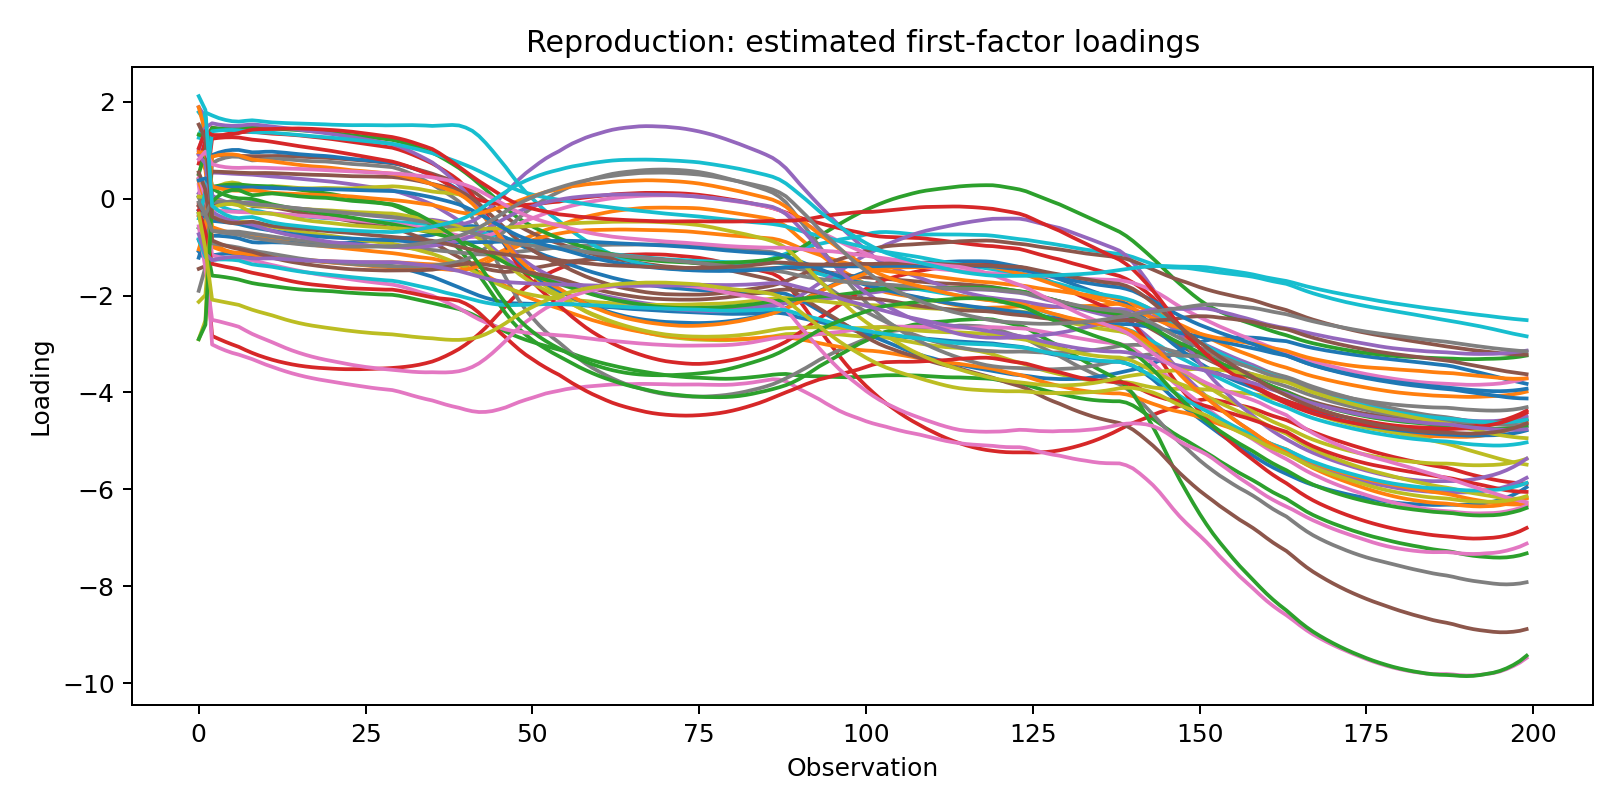
\includegraphics[width=\linewidth]{reproduction_factor_loadings.png}
  \caption{Estimated first-factor loading paths.}
\end{subfigure}
\hfill
\begin{subfigure}{0.49\textwidth}
  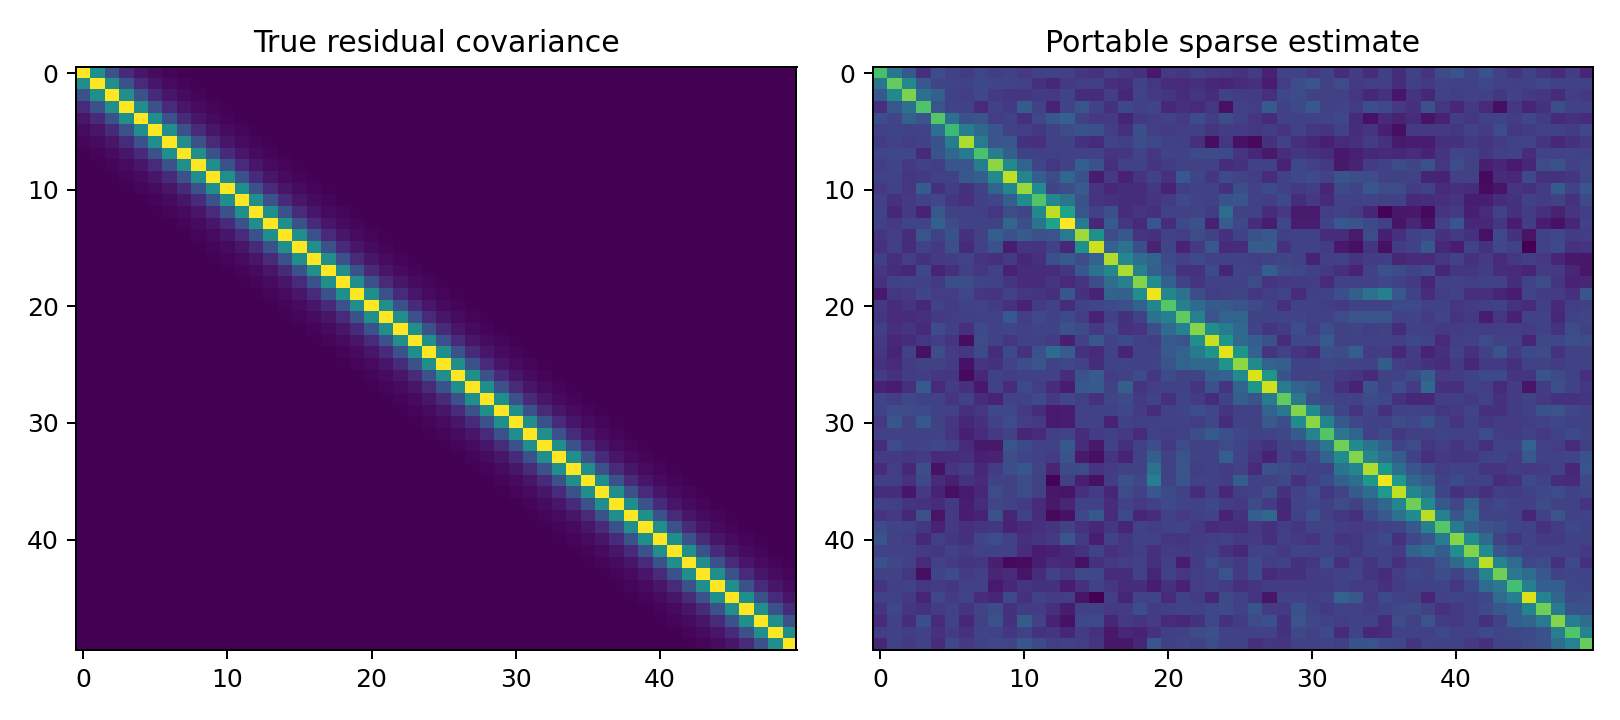
\includegraphics[width=\linewidth]{reproduction_residual_covariance.png}
  \caption{True and portable residual covariance.}
\end{subfigure}
\caption{Reproduction diagnostics. Loading trajectories are visibly time-varying, while portable thresholding recovers broad residual-covariance structure but not the author's exact penalised estimator.}
\label{fig:reproduction}
\end{figure}

\section{Extension 1: dynamic factor covariance}

\subsection{Motivation}

Equation \eqref{eq:base-cov} treats the factor covariance as constant across the complete rolling window. If the volatility of common shocks rises or falls faster than the loading functions, equal weighting of historical scores can lag. The minimal extension changes only the factor covariance term, leaving local loadings and sparse residual covariance untouched. This makes C a clean diagnostic of whether recency-weighted factor risk adds value beyond time-varying exposures.

\subsection{EWMA estimator}

For decay $\lambda\in(0,1)$ and $T$ estimated score vectors, define
\begin{equation}
 a_t=\frac{\lambda^{T-t}}{\sum_{j=1}^T\lambda^{T-j}},
 \qquad \bar f_a=\sum_{t=1}^T a_t\wh f_t.
\end{equation}
The weighted covariance includes the finite-weight degrees correction
\begin{equation}
 \wh\Sigma_{F,T}^{\text{EWMA}}
 =\frac{\sum_{t=1}^Ta_t(\wh f_t-\bar f_a)(\wh f_t-\bar f_a)\trans}
 {1-\sum_{t=1}^Ta_t^2}.
 \label{eq:ewma}
\end{equation}
The effective number of observations is
\begin{equation}
 T_{\text{eff}}=\left(\sum_ta_t^2\right)^{-1}.
\end{equation}
With $lambda=0.94$ and $T=504$, $T_{\text{eff}}=32.33$. Thus the extension reacts quickly but estimates factor covariance from an amount of information comparable to only 32 equally weighted observations. This variance-bias trade-off is central to interpreting the weak empirical improvement.

\section{Extension 2: scenario-based CVaR}

\subsection{Loss, VaR, and expected shortfall}

For portfolio return $R_p=w\trans r$, define loss $L=-R_p$. At confidence $\beta$,
\begin{equation}
 \VaR_\beta(L)=\inf\{\ell:\Pr(L\le\ell)\ge\beta\}.
\end{equation}
For continuous losses, expected shortfall is
\begin{equation}
 \ES_\beta(L)=\E[L\mid L\ge\VaR_\beta(L)].
\end{equation}
Expected shortfall is a coherent tail-risk measure under standard definitions \cite{acerbitasche2002}. Rockafellar and Uryasev express CVaR through the convex function \cite{rockafellar2000,rockafellar2002}
\begin{equation}
 \Phi_\beta(w,\alpha)=\alpha+\frac{1}{1-\beta}\E[(L(w)-\alpha)_+].
 \label{eq:ru-pop}
\end{equation}
Minimising \eqref{eq:ru-pop} jointly over $w$ and $\alpha$ minimises CVaR; $\alpha$ acts as a VaR threshold.

\subsection{Baseline scenario generator}

At each rebalance, only the trailing fitted scores $\{\wh f_t\}$, residual vectors $\{\wh e_t\}$, and current endpoint loading $\wh B_T$ are available. A circular moving-block bootstrap chooses a uniform start index and appends $L=10$ consecutive paired observations, wrapping at the sample end, until $S=600$ scenario dates are obtained. Scores and residual vectors use the same indices, preserving their contemporaneous empirical relationship and short-run time ordering. Scenario $s$ is
\begin{equation}
 r^{(s)}=\wh B_T\wh f_{J_s}+\wh e_{J_s}.
 \label{eq:baseline-scenario}
\end{equation}
This generator is empirical: it can rearrange historical blocks but cannot create a shock magnitude absent from the 504-day window. It also maps all past factors through today's loading while leaving historical score and residual scales unfiltered.

\subsection{Finite-scenario linear program}

For scenario returns $r^{(s)}$ and $\beta=0.95$, the baseline optimisation is
\begin{align}
 \min_{w,\alpha,u}\quad &\alpha+\frac{1}{(1-\beta)S}\sum_{s=1}^S u_s,\label{eq:cvar-lp}\\
 \text{s.t.}\quad
 &u_s\ge-r^{(s)\trans}w-\alpha,\quad u_s\ge0,\\
 &\one\trans w=1,\quad 0\le w_i\le0.10.
\end{align}
It is solved with SciPy HiGHS. At 95\% and 600 scenarios, only roughly 30 observations lie in the nominal tail. Block dependence makes the effective amount of independent tail information smaller still. An optimiser can exploit accidental differences among these few tail observations, producing unstable corner portfolios even when the LP is solved exactly.

\subsection{Why CVaR need not maximise return}

Program \eqref{eq:cvar-lp} contains no expected-return term. A stock that avoided losses in the fitted tail can receive weight even if it has weak subsequent upside. Conversely, a stock with high expected return but several historical losses is penalised. CVaR is not ``wrong'' when such a portfolio lags a rally; it is optimising a different functional. The meaningful failure occurs when it also fails on realised tail loss, which is what the matched post-2021 experiment finds.

\section{Filtered, stressed, and regularised CVaR}

\subsection{Filtered historical innovations}

Let $S_f$ and $S_e$ be the unweighted sample covariances of centred fitted scores and residuals. Symmetric whitening produces
\begin{equation}
 z^f_t=(\wh f_t-\bar f)S_f^{-1/2},
 \qquad z^e_t=(\wh e_t-\bar e)S_e^{-1/2}.
\end{equation}
Small eigenvalues are floored before inverse square roots. Current target factor covariance is Equation \eqref{eq:ewma}. Current residual covariance is
\begin{equation}
 Q_{e,T}=\omega\wh\Sigma_{e,T}^{\text{EWMA}}
 +(1-\omega)\wh\Sigma_e^{\text{sparse}},
 \qquad \omega=0.50,
 \label{eq:residual-blend}
\end{equation}
where residual EWMA decay is 0.97. The mixture is repaired to be positive definite.

Circular block starts now have probability
\begin{equation}
 \pi_j=\frac{\delta^{T-1-j}}{\sum_{q=0}^{T-1}\delta^q},
 \qquad \delta=0.995,
\end{equation}
so recent blocks are more likely. Pairing remains intact. With $S=800$ and stress indicator $I_s\sim\operatorname{Bernoulli}(0.15)$, the filtered scenario is
\begin{equation}
 r^{(s)}=\wh B_T\left[m_f(I_s)z^f_{J_s}Q_{f,T}^{1/2}\right]
 +m_e(I_s)z^e_{J_s}Q_{e,T}^{1/2},
 \label{eq:filtered-scenario}
\end{equation}
where $m_f(0)=m_e(0)=1$, $m_f(1)=1.50$, and $m_e(1)=1.15$. Because common-factor shocks receive the larger multiplier, stressed draws increase the common component's share of total variance and thereby tend to raise cross-asset correlation as well as volatility. This is a transparent stress mixture, not an estimated regime-transition probability.

\subsection{Regularised CVaR objective}

The final variant solves
\begin{equation}
 \min_{w,\alpha,u}\quad
 \wh\CVaR_{0.95}(w)
 +\eta_{\text{turn}}\|w-w^-\|_1
 +\eta_{\text{div}}\left\|w-\frac{1}{p}\one\right\|_1,
 \label{eq:regularized-cvar}
\end{equation}
subject to Equation \eqref{eq:matched-constraints}, with $\eta_{\text{turn}}=0.0010$ and $\eta_{\text{div}}=0.00025$. Here $w^-$ is the naturally drifted pre-trade portfolio. Auxiliary nonnegative variables linearise both absolute-value penalties, so the entire problem remains a linear program.

The first penalty makes small forecast changes insufficient to trigger large trades. The second shrinks toward equal weight and discourages needless zeros and cap hits. It is an $L_1$ distance penalty, not a direct penalty on the Herfindahl index; ``diversification regularisation'' should therefore be read as shrinkage toward $1/p$.

\subsection{Positive-definite repair}
\label{sec:pd}

Every covariance is symmetrised, eigendecomposed, and floored:
\begin{equation}
 A=Q\operatorname{diag}(d_1,\ldots,d_p)Q\trans,
 \quad
 \widetilde A=Q\operatorname{diag}\big(\max(d_i,\varepsilon s)\big)Q\trans,
\end{equation}
where $s=\max(\max_i|d_i|,1)$ and $\varepsilon=10^{-7}$. The number of clipped eigenvalues and before/after minima are returned for audit. In the empirical core diagnostics, no factor or residual covariance eigenvalues required clipping. Whitening separately uses a numerical floor of $10^{-12}$.

\section{Backtest accounting and performance measures}

\subsection{Holdings drift and turnover}

If target weight $w_{i,0}$ is held through asset return $r_{i,t}$, the post-return weight is
\begin{equation}
 w^-_{i,t}=\frac{w_{i,t-1}(1+r_{i,t})}{1+w_{t-1}\trans r_t}.
\end{equation}
At rebalance $j$, reported one-way turnover is
\begin{equation}
 \operatorname{TO}_j=\frac12\|w_j-w^-_j\|_1.
\end{equation}
The code charges $c\|w_j-w^-_j\|_1=2c\operatorname{TO}_j$ on the first holding day, with $c=10$ basis points for each unit of gross bought-or-sold notional. Inception turnover is set to zero, so initial establishment cost is omitted. Annualised turnover is total one-way turnover divided by out-of-sample years.

\subsection{Return and risk definitions}

For daily returns $x_1,\ldots,x_n$ and $A=252$:
\begin{align}
 \text{annualised geometric return}
 &=\left[\prod_{t=1}^n(1+x_t)\right]^{A/n}-1,\\
 \text{annualised volatility}
 &=\sqrt A\,\operatorname{sd}(x_t),\\
 \text{Sharpe-like ratio}
 &=\sqrt A\,\frac{\bar x}{\operatorname{sd}(x_t)},\\
 \text{maximum drawdown}
 &=\min_t\left(\frac{W_t}{\max_{s\le t}W_s}-1\right),\\
 \text{reported daily ES}
 &=\sqrt A\,\frac{1}{|\mathcal T|}\sum_{t\in\mathcal T}(-x_t),
\end{align}
where $W_t=\prod_{s\le t}(1+x_s)$ and $\mathcal T$ contains losses at or above the empirical 95th percentile. Sharpe uses gross returns in the main performance table, while ``net return'' uses returns after transaction costs.

\warningBox{Multiplying daily empirical ES by $\sqrt{252}$ is a reporting convention, not an exact temporal aggregation law. It is exact only under restrictive scale-stable assumptions. The formal comparison therefore also works directly with non-overlapping monthly portfolio losses.}

\section{Statistical analysis}

\subsection{Monthly paired moving-block bootstrap}

Daily net portfolio returns are compounded within calendar month:
\begin{equation}
 R_{m,k}=\prod_{t\in m}(1+r^{\text{net}}_{t,k})-1,
 \qquad L_{m,k}=-R_{m,k}.
\end{equation}
For strategies $a$ and $b$, the statistics are differences in annualised monthly-loss volatility, monthly ES, and annualised geometric net return:
\begin{align}
 \Delta_\sigma&=\sqrt{12}\,[\operatorname{sd}(L_a)-\operatorname{sd}(L_b)],\\
 \Delta_{ES}&=\ES_{0.95}(L_a)-\ES_{0.95}(L_b),\\
 \Delta_R&=R^{\text{ann}}_a-R^{\text{ann}}_b.
\end{align}

Each bootstrap draw samples circular blocks of three consecutive months until the original number of months is reached. The same month indices are applied to every strategy, preserving paired cross-strategy shocks and short-run serial dependence \cite{kunsch1989}. The project uses 1,999 draws and percentile 95\% intervals.

The reported two-sided bootstrap probability is
\begin{equation}
 p^*=2\min\{\Pr^*(\Delta^*\le0),\Pr^*(\Delta^*\ge0)\},
 \label{eq:bootstrap-p}
\end{equation}
capped at one. It is shown only for pre-specified pairs. This is a sign-probability from the uncentred bootstrap distribution, not a studentised null-recentred test. It is useful descriptive evidence, but a journal submission should add a formally null-imposed block-bootstrap or studentised procedure.

Core primary comparisons were B versus C and C versus D. Matched primary comparisons were matched B versus D and matched C versus D. Improved-run primary comparisons were empirical D versus D-FS and matched B versus D-REG. All other pairwise intervals are exploratory and deliberately have missing p-values. No family-wise or false-discovery adjustment is applied; robustness sweeps are not treated as hypothesis tests.

\subsection{Ex-ante volatility regimes}

Regimes use the NIFTY index, never portfolio outcomes. Let
\begin{equation}
 v_t=\sqrt{252}\,\operatorname{sd}(r^{\text{index}}_{t-20:t}).
\end{equation}
The signal is shifted one day. The threshold is the expanding historical 75th percentile of the shifted signal, requiring at least 126 observations and itself shifted once more. Day $t$ is high volatility when yesterday's known $v$ exceeds the threshold known before day $t$. Missing early classifications default to normal.

The core interaction asks whether C's risk benefit over B is larger in high volatility:
\begin{equation}
 [M(B,H)-M(C,H)]-[M(B,N)-M(C,N)],
\end{equation}
for volatility and ES. The improved interaction analogously compares regularised CVaR with empirical CVaR and adds arithmetic annualised net return. Circular daily blocks have length 21 and use 1,999 draws.

\subsection{Covariance forecast quality}

For rebalance $j$, the realised proxy is the sample covariance of daily asset returns over the next monthly holding interval, $\Sigma^{\text{real}}_{j+1}$. Two losses are
\begin{align}
 \mathcal L_F&=\|\wh\Sigma_j-\Sigma^{\text{real}}_{j+1}\|_F,\\
 \mathcal L_w&=\left|w_j\trans\Sigma^{\text{real}}_{j+1}w_j-w_j\trans\wh\Sigma_jw_j\right|.
\end{align}
The first evaluates the whole matrix; the second evaluates forecast error along the selected portfolio direction. The realised proxy is noisy because each month contains only about 20 observations for 39 assets. In simulation, the future true covariance is known and averaged across the 63-day evaluation interval.

\subsection{Factor diagnostics}

At each rebalance the project records:
\begin{enumerate}
  \item retained variance share: sum of the first $K$ weighted singular values squared divided by the sum over all singular values;
  \item loading-space stability: the largest principal angle between consecutive endpoint loading column spaces;
  \item residual-correlation sparsity: fraction of off-diagonal thresholded correlations equal to zero;
  \item Fisher excess kurtosis of each factor score series, averaged across factors;
  \item median Fisher excess kurtosis across residual series;
  \item eigenvalue clipping counts and EWMA effective sample size.
\end{enumerate}
The final-window standardised factors and residuals receive normal QQ plots. No large-sample omnibus normality-test p-values are used because tiny deviations become mechanically significant at large sample sizes.

\section{Empirical results}

\subsection{Core full-sample comparison}

\begin{table}[H]
\centering
\caption{Core NIFTY results, February 2017--August 2026}
\label{tab:core-results}
\resizebox{\textwidth}{!}{%
\begin{tabular}{@{}lrrrrrrrr@{}}
\toprule
Model & Gross return & Volatility & Sharpe & Max DD & ES 95\% & Turnover & Net return & Net wealth \\
\midrule
Equal weight & 19.81\% & 15.94\% & 1.215 & -35.79\% & 36.86\% & 0.31 & 19.74\% & 5.411 \\
Original TV-MVP & 15.88\% & 14.37\% & 1.098 & -30.04\% & 31.81\% & 6.63 & 14.35\% & 3.515 \\
Dynamic-$\Sigma_F$ TV-MVP & 15.74\% & 14.36\% & 1.091 & -30.34\% & 31.81\% & 6.63 & 14.22\% & 3.477 \\
Dynamic-factor CVaR & 13.44\% & 14.19\% & 0.960 & -34.37\% & 31.65\% & 4.73 & 12.37\% & 2.983 \\
\bottomrule
\end{tabular}}
\end{table}

The dynamic factor covariance is nearly indistinguishable from the original. CVaR has slightly lower daily volatility and ES than the unconstrained original, but this comparison mixes objective and feasible-set effects. Equal weight's large drawdown shows that its high return and Sharpe did not imply lower downside magnitude.

\begin{figure}[H]
\centering
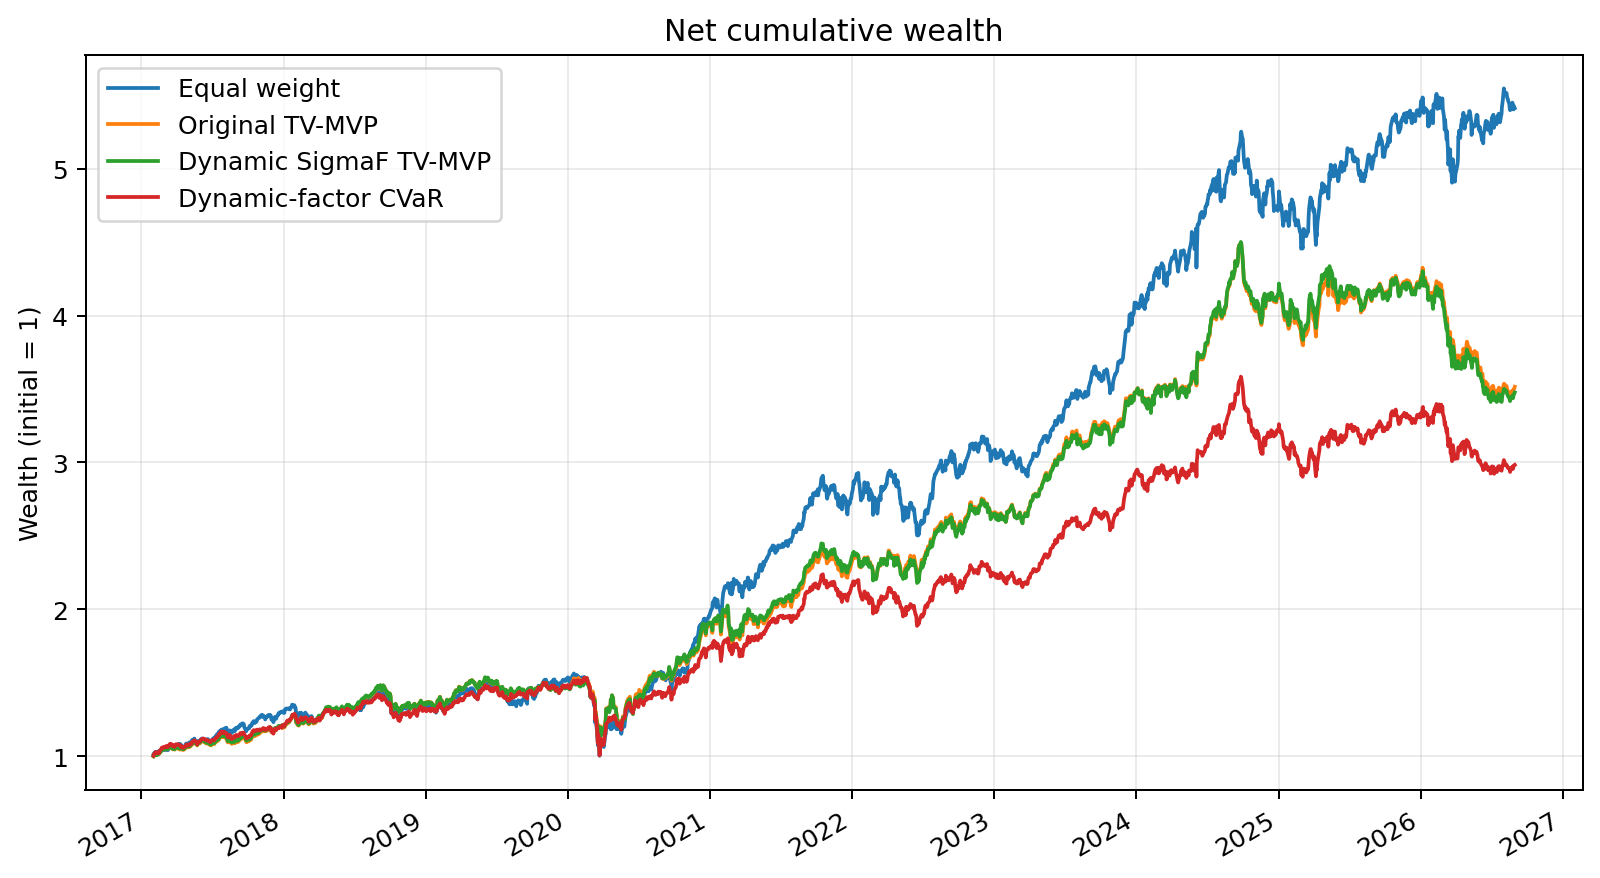
\includegraphics[width=0.92\textwidth]{cumulative_net_returns.png}
\caption{Full-sample cumulative net wealth for the core comparison.}
\label{fig:cumulative}
\end{figure}

\subsection{Primary monthly inference}

\begin{table}[H]
\centering
\caption{Pre-specified core comparisons using monthly losses}
\label{tab:core-inference}
\begin{tabularx}{\textwidth}{@{}llrrrr@{}}
\toprule
Pair (1 minus 2) & Metric & Estimate & CI low & CI high & $p^*$ \\
\midrule
B minus C & Ann. volatility & 0.00038 & -0.00198 & 0.00238 & 0.755 \\
B minus C & Monthly ES & 0.00198 & -0.00580 & 0.00901 & 0.434 \\
B minus C & Ann. net return & 0.00131 & -0.00766 & 0.01089 & 0.781 \\
C minus D & Ann. volatility & -0.00701 & -0.02382 & 0.01072 & 0.498 \\
C minus D & Monthly ES & -0.01492 & -0.03600 & 0.00183 & 0.119 \\
C minus D & Ann. net return & 0.01804 & -0.01883 & 0.05471 & 0.358 \\
\bottomrule
\end{tabularx}
\end{table}

All intervals contain zero. Nothing in the full-sample primary inference supports a statistically distinguishable advantage for dynamic $\Sigma_F$ or baseline CVaR.

\subsection{Regime results}

High-volatility days number 560; normal-volatility days number 1,802. B and C have virtually identical high-regime volatility (22.30\%) and ES (53.16\% versus 53.13\%). D has 21.75\% volatility and 50.72\% ES in the high regime, but lower normal-regime return and Sharpe. The high-minus-normal dynamic-covariance benefit is -0.00018 for volatility (95\% CI -0.00404, 0.00396; $p^*=0.906$) and 0.00103 for ES (CI -0.01585, 0.01734; $p^*=0.975$). There is no evidence that extension C becomes more useful when index volatility is high.

\begin{figure}[H]
\centering
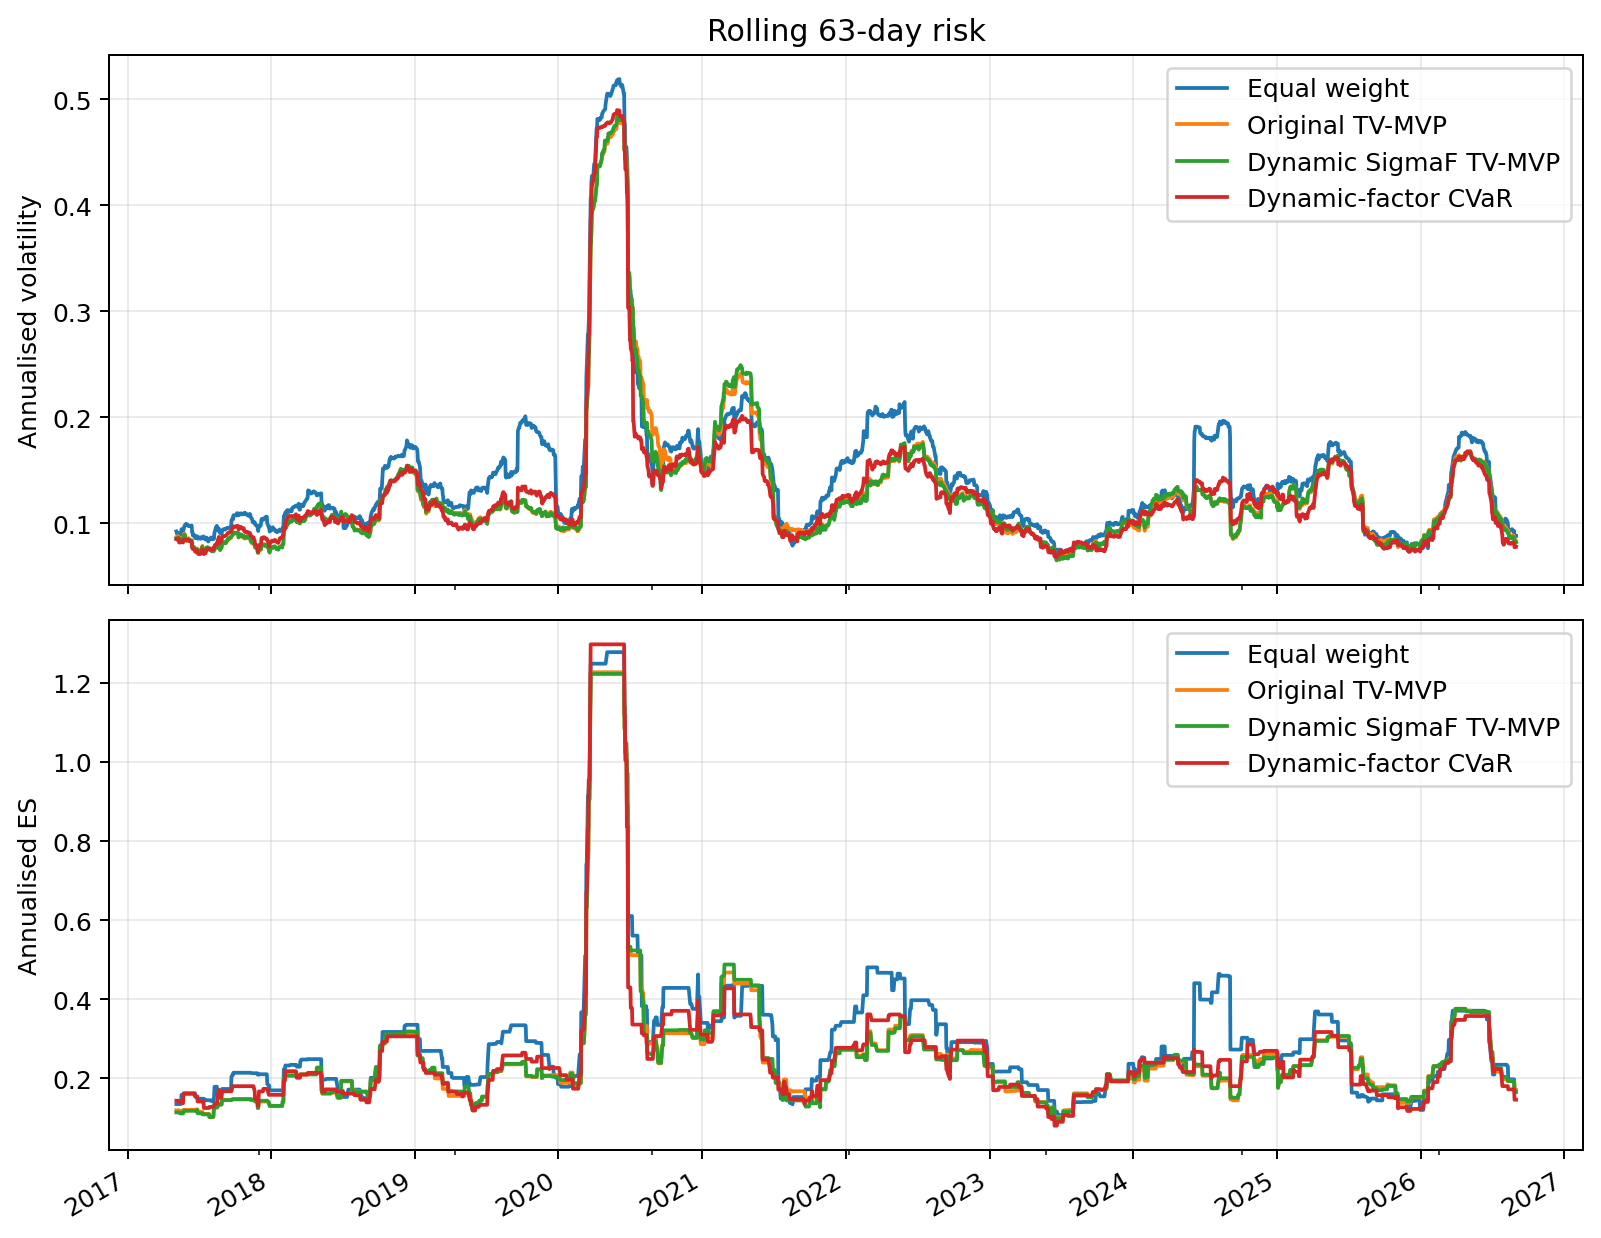
\includegraphics[width=0.92\textwidth]{rolling_volatility_es.png}
\caption{Rolling 63-day annualised volatility and empirical ES. The common temporal movement dominates the modest cross-strategy differences.}
\label{fig:rolling-risk}
\end{figure}

\subsection{Covariance forecast evaluation}

\begin{table}[H]
\centering
\caption{Mean next-holding-period covariance forecast losses}
\label{tab:cov-loss}
\begin{tabular}{@{}lrr@{}}
\toprule
Model & Frobenius loss & Portfolio-risk loss \\
\midrule
Original TV-MVP & 0.005623 & 0.000057 \\
Dynamic-$\Sigma_F$ TV-MVP & 0.005958 & 0.000058 \\
CVaR scenario covariance & 0.005573 & 0.000052 \\
\bottomrule
\end{tabular}
\end{table}

Dynamic factor covariance does not improve either mean loss. The CVaR scenario covariance has slightly smaller averages, yet its portfolio is not better after matching constraints. A globally good covariance approximation does not guarantee accurate estimation of a small tail functional, and portfolio optimisation can amplify local forecast errors.

\subsection{Factor-model diagnostics}

Three factors explain 48.91\% of locally weighted variation on average, ranging from 35.38\% to 76.78\%. Consecutive loading subspaces have a mean maximum principal angle of 54.48 degrees and a maximum of 89.98 degrees, indicating substantial endpoint instability. Only 14.47\% of off-diagonal residual correlations are exactly thresholded to zero. Mean factor excess kurtosis is 2.43; median residual excess kurtosis is 2.49. These values and the QQ plots demonstrate much heavier tails than Gaussian benchmarks.

\begin{figure}[H]
\centering
\begin{subfigure}{0.49\textwidth}
  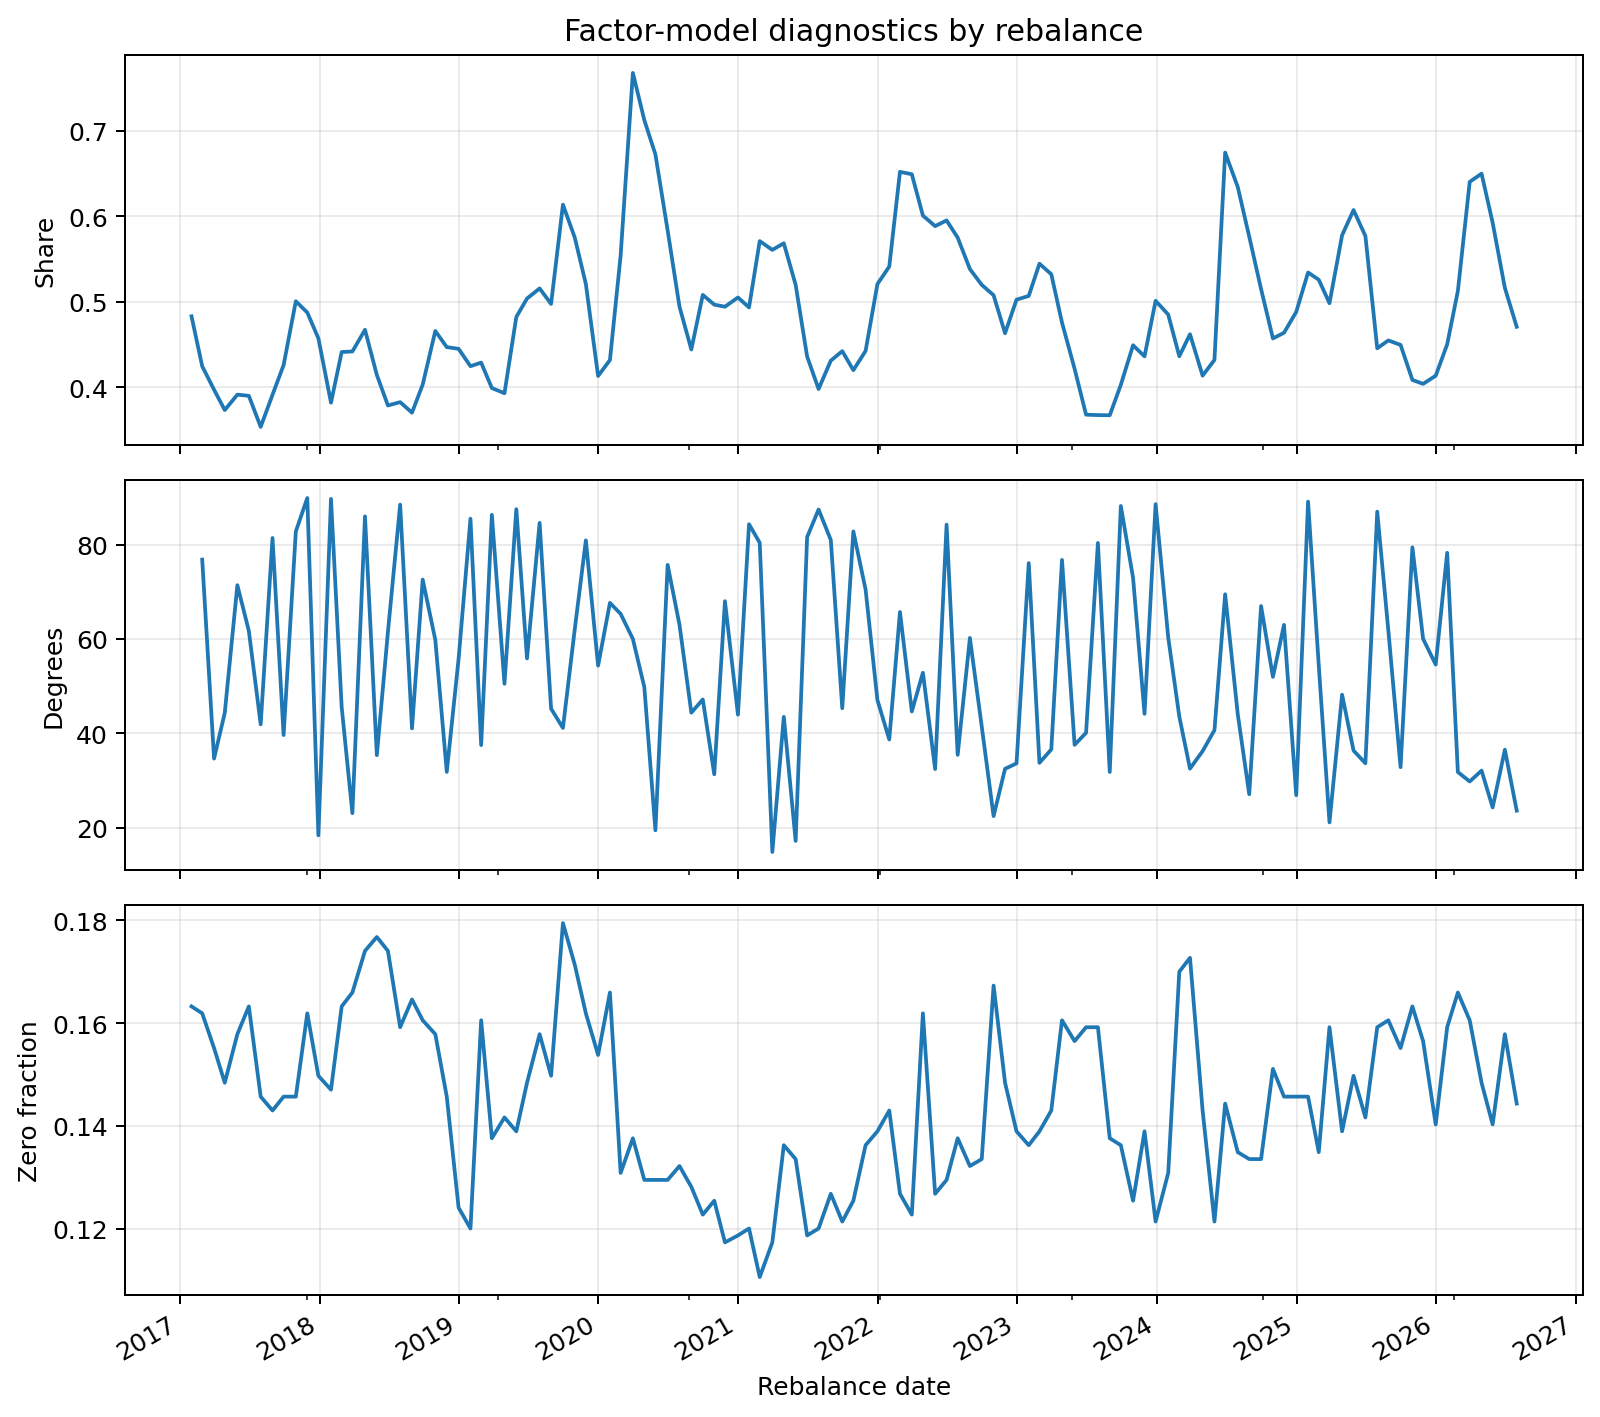
\includegraphics[width=\linewidth]{factor_diagnostics.png}
  \caption{Explained variance, loading angle, and sparsity.}
\end{subfigure}
\hfill
\begin{subfigure}{0.49\textwidth}
  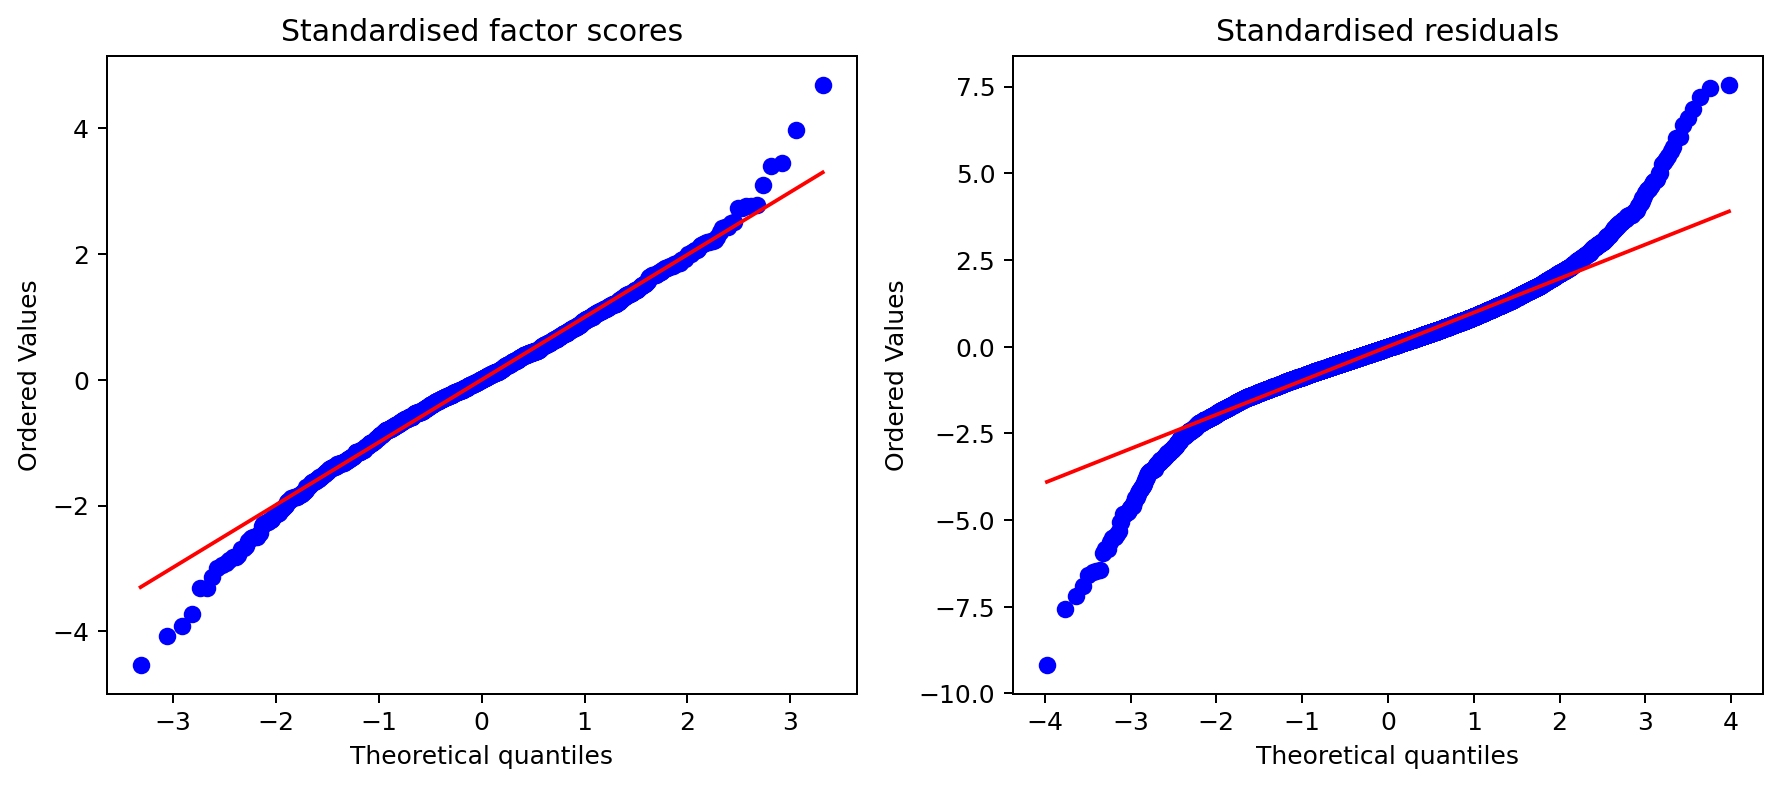
\includegraphics[width=\linewidth]{factor_residual_qq.png}
  \caption{Final-window standardised QQ plots.}
\end{subfigure}
\caption{Factor diagnostics. Large principal angles and heavy-tailed scores/residuals are directly relevant to covariance and CVaR instability.}
\label{fig:factor-diag}
\end{figure}

\section{Why empirical CVaR failed after 2021}

\subsection{Removing the feasible-set confound}

The original post-2021 comparison was partly confounded: B was unconstrained whereas D was long-only and capped. The matched rerun applies Equation \eqref{eq:matched-constraints} to both MVP estimators and CVaR.

\begin{table}[H]
\centering
\caption{Matched post-2021 comparison}
\label{tab:matched}
\resizebox{\textwidth}{!}{%
\begin{tabular}{@{}lrrrrrrr@{}}
\toprule
Model & Gross return & Net return & Volatility & Sharpe & Max DD & ES 95\% & Turnover \\
\midrule
Equal weight & 20.14\% & 20.07\% & 13.87\% & 1.393 & -15.15\% & 32.09\% & 0.29 \\
Original-covariance MVP & 13.62\% & 12.79\% & 11.86\% & 1.136 & -17.13\% & 26.17\% & 3.69 \\
Dynamic-covariance MVP & 13.52\% & 12.62\% & 11.92\% & 1.123 & -16.63\% & 26.25\% & 3.99 \\
Empirical CVaR & 11.22\% & 10.17\% & 12.13\% & 0.937 & -18.68\% & 27.23\% & 4.75 \\
\bottomrule
\end{tabular}}
\end{table}

Under the same constraints, empirical CVaR is worse than original MVP on every displayed measure. The monthly block-bootstrap comparison B minus D gives annualised volatility difference -0.00862 (CI -0.01522, -0.00219; $p^*=0.010$), monthly ES difference -0.01061 (CI -0.01944, -0.00139; $p^*=0.031$), and annualised net return difference 0.02565 (CI 0.00083, 0.05109; $p^*=0.043$). Within this sample and test definition, matched B is distinguishable at 5\% on all three registered measures.

\subsection{Forecast-tail reversal}

Empirical CVaR succeeds inside its fitted scenario distribution: mean fitted daily CVaR is 1.106\%, below matched original MVP's 1.226\%. Out of sample, the ordering reverses: realised holding-period daily CVaR averages 1.326\% for D and 1.295\% for B. D's fitted-to-realised gap is 0.219 percentage point, its VaR exceedance rate is 10.25\%, and its forecast/realised CVaR rank correlation is only 0.314.

This pattern distinguishes three explanations:
\begin{enumerate}
  \item \textbf{Not a solver bug:} the LP finds a portfolio with lower objective value in the supplied scenarios.
  \item \textbf{Not merely the cap:} the reversal remains when MVP has the same cap and long-only rules.
  \item \textbf{Scenario/optimisation interaction:} a small, under-responsive empirical tail is treated as known, and the optimiser magnifies its sampling error.
\end{enumerate}

\subsection{Corner solutions and costs}

Baseline CVaR holds 12.52 effective assets on average, places 4.91 weights at the cap, and sets 22.51 of 39 weights to zero. Matched original MVP holds 14.23 effective assets, with 3.18 cap hits and 18.99 zeros. D's annual turnover is 4.75 versus B's 3.69. The gross return gap already exists, so costs are not the sole cause; costs widen it.

\begin{figure}[H]
\centering
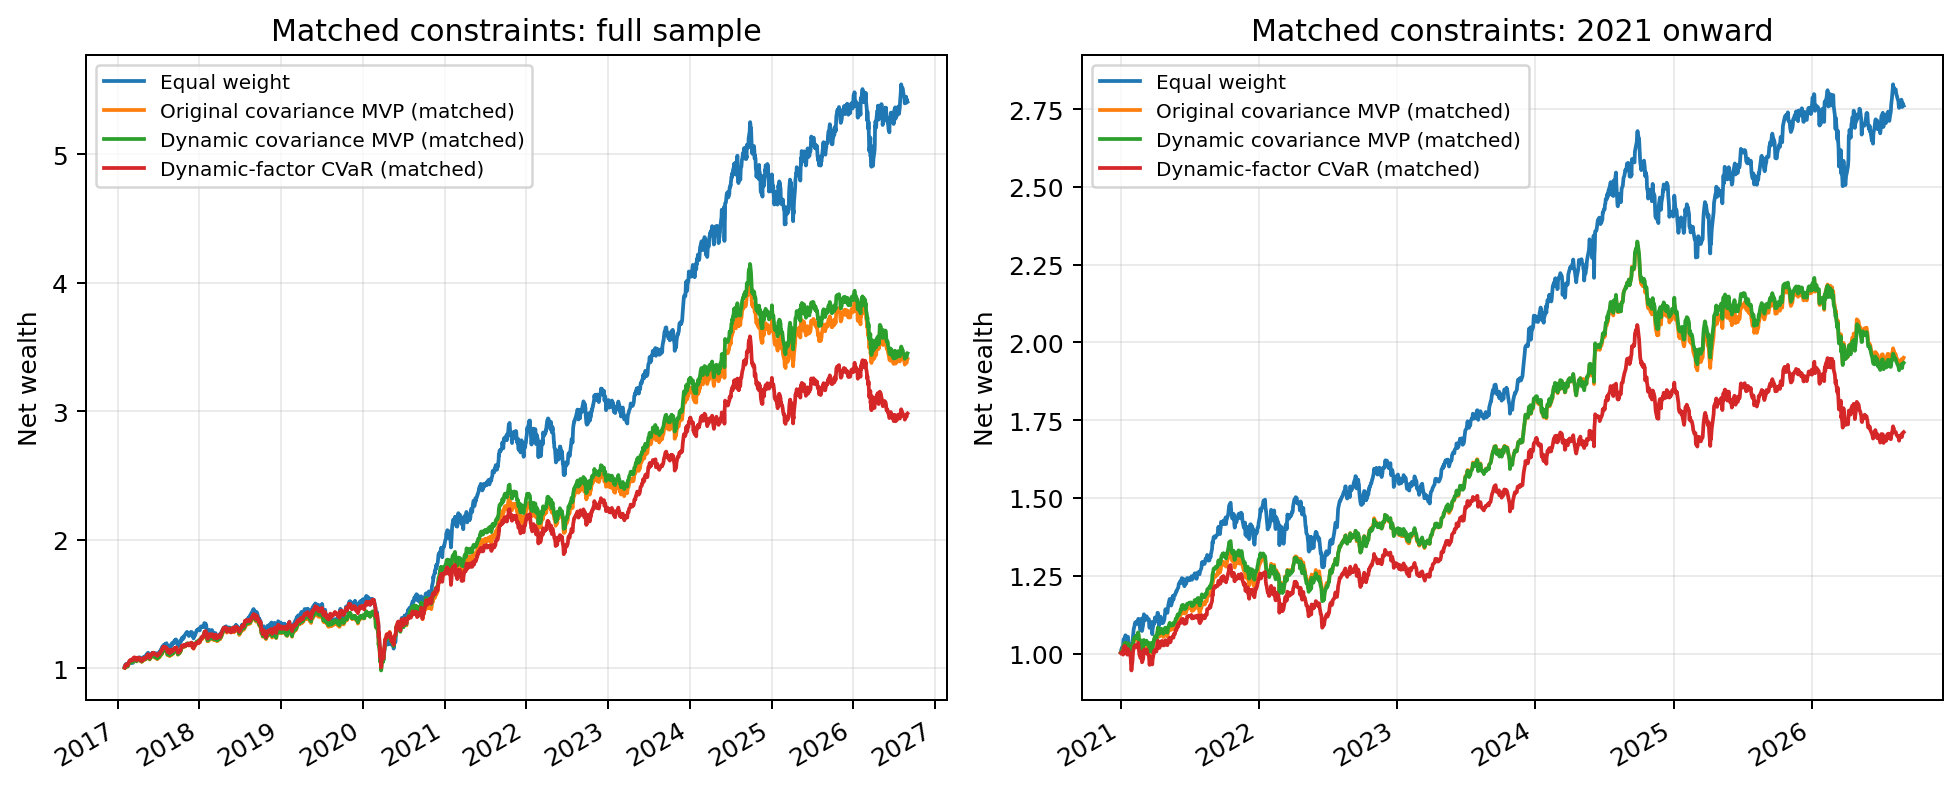
\includegraphics[width=0.94\textwidth]{matched_constraint_returns.png}
\caption{Cumulative net wealth for the matched-constraint experiment, over the full period and after 2021.}
\label{fig:matched-return}
\end{figure}

\section{Improved CVaR results}

\subsection{Ablation results}

\begin{table}[H]
\centering
\caption{Post-2021 improved-CVaR ablation; all optimisers matched}
\label{tab:improved}
\resizebox{\textwidth}{!}{%
\begin{tabular}{@{}lrrrrrrr@{}}
\toprule
Model & Gross return & Net return & Volatility & Sharpe & Max DD & ES 95\% & Turnover \\
\midrule
Original-covariance MVP & 13.62\% & 12.79\% & 11.86\% & 1.136 & -17.13\% & 26.17\% & 3.69 \\
Empirical CVaR & 11.22\% & 10.17\% & 12.13\% & 0.937 & -18.68\% & 27.23\% & 4.75 \\
Filtered/stressed CVaR & 13.92\% & 12.88\% & 12.10\% & 1.138 & -16.94\% & 27.00\% & 4.60 \\
Regularised filtered CVaR & 15.10\% & 14.30\% & 11.95\% & 1.237 & -15.67\% & 26.56\% & 3.50 \\
\bottomrule
\end{tabular}}
\end{table}

Filtering and stressing add 2.71 percentage points of annualised net return relative to empirical CVaR, with nearly unchanged daily volatility and a 0.23-point reduction in annualised daily ES. Adding regularisation contributes another 1.42 points of net return, reduces volatility by 0.15 point, improves maximum drawdown by 1.27 points, reduces ES by 0.44 point, and removes 1.10 units of annual turnover.

Relative to matched original MVP, D-REG has 1.51 points higher net return, a 0.100 higher Sharpe ratio, and a 1.46-point shallower maximum drawdown. It also has 0.09 point higher daily volatility and 0.39 point higher annualised daily ES. Thus even the point-estimate verdict depends on the performance measure.

\subsection{Calibration after the repair}

\begin{table}[H]
\centering
\caption{Post-2021 tail calibration and concentration}
\label{tab:calibration}
\resizebox{\textwidth}{!}{%
\begin{tabular}{@{}lrrrrrr@{}}
\toprule
Model & Scenario CVaR & Realised CVaR & Gap & Exceedance & Rank corr. & Effective assets \\
\midrule
Empirical CVaR & 0.01106 & 0.01326 & 0.00219 & 10.25\% & 0.314 & 12.52 \\
Filtered/stressed CVaR & 0.01286 & 0.01309 & 0.00023 & 8.63\% & 0.446 & 12.06 \\
Regularised filtered CVaR & 0.01282 & 0.01287 & 0.00005 & 8.14\% & 0.446 & 12.56 \\
Matched original MVP$^\dagger$ & 0.01431 & 0.01295 & -0.00136 & 7.13\% & 0.451 & 14.23 \\
\bottomrule
\end{tabular}}
\vspace{0.3em}
\begin{minipage}{0.94\textwidth}\footnotesize
$^\dagger$For the improved diagnostic, non-empirical-CVaR models are evaluated on the same filtered/stressed scenario system. Scenario CVaR is a forecast diagnostic for MVP, not its optimisation objective.
\end{minipage}
\end{table}

The stress mixture removes most average underprediction and increases rank correlation, but exceedance remains well above the nominal 5\%. The filtered optimiser alone becomes slightly more concentrated; most of the trading improvement comes from explicit regularisation, not from filtering automatically creating diversified weights.

\subsection{Statistical uncertainty}

For the pre-specified empirical-D minus D-FS comparison, annualised monthly volatility difference is 0.00470 (CI -0.00458, 0.01425; $p^*=0.315$), monthly ES difference is 0.01408 (CI -0.00080, 0.02552; $p^*=0.071$), and annualised net-return difference is -0.02650 (CI -0.05916, 0.00365; $p^*=0.097$). These are suggestive but not 5\%-significant.

For matched B minus D-REG, annualised monthly volatility difference is -0.00451 (CI -0.01182, 0.00255; $p^*=0.221$), monthly ES difference is 0.00258 (CI -0.00513, 0.00902; $p^*=0.497$), and annualised net-return difference is -0.01473 (CI -0.04282, 0.01151; $p^*=0.275$). None is statistically distinguishable from zero.

Exploratory empirical-D minus D-REG intervals exclude zero for monthly ES and annualised net return, but that pair was not designated primary and receives no p-value. This protects the analysis from relabelling the most favourable post-hoc pair as confirmatory.

\subsection{High- versus normal-volatility performance}

After 2021, 313 days are classified high volatility and 1,086 normal. In high volatility, empirical D versus D-REG has volatility 16.05\% versus 16.13\%, and ES 33.69\% versus 32.83\%. In normal volatility, the corresponding figures are 10.71\% versus 10.41\%, and 24.91\% versus 23.76\%. The 21-day-block interaction test does not show a larger high-regime benefit: volatility interaction -0.00377 ($p^*=0.234$), ES interaction -0.00292 ($p^*=0.740$), and arithmetic net-return interaction 0.01547 ($p^*=0.665$).

\begin{figure}[H]
\centering
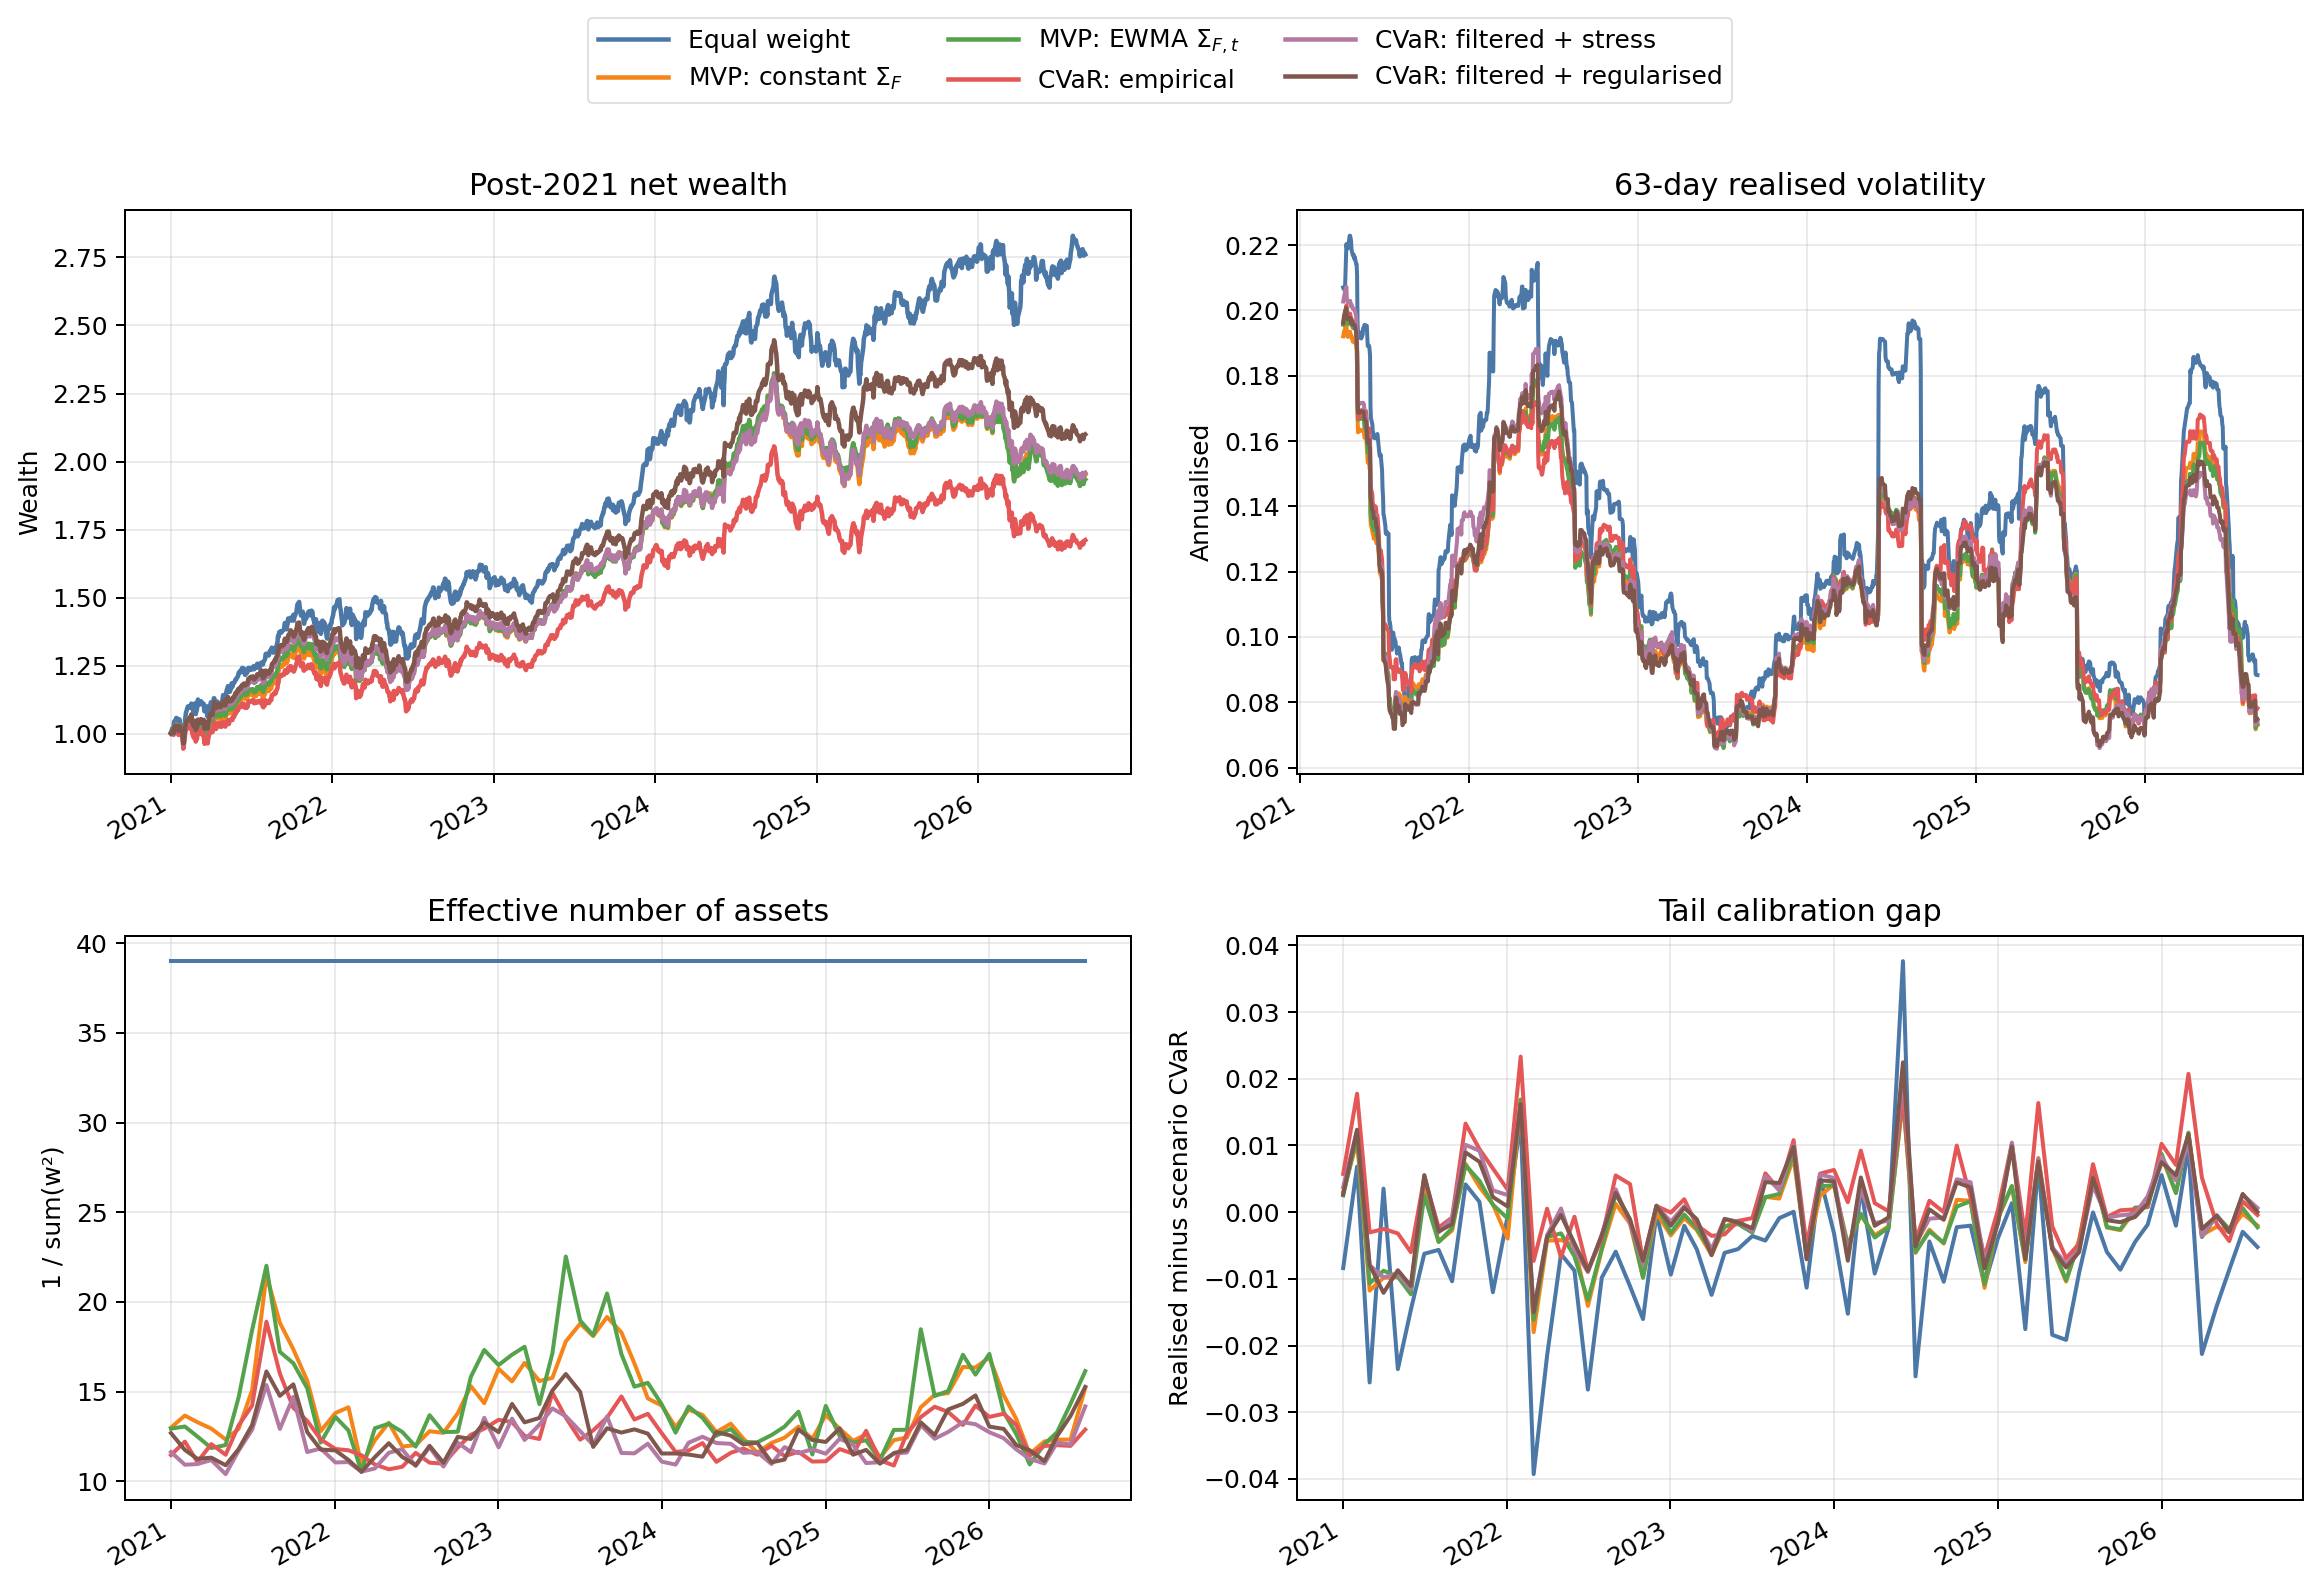
\includegraphics[width=\textwidth]{improved_cvar_diagnostics.png}
\caption{Post-2021 improved-CVaR diagnostics. The shared legend identifies all six series. Regularised filtered CVaR improves wealth and turnover-related stability, but risk paths remain close and calibration gaps still spike in some months.}
\label{fig:improved-diag}
\end{figure}

\section{Simulation evidence}

\subsection{Design}

Each of three settings has 100 independent replications, with fixed but changeable project seed, $p=20$, $K=2$, 180 estimation days, and 63 evaluation days. Loadings evolve smoothly:
\begin{equation}
 B_t=B_0+D\sin(2\pi t/(T+H-1)).
\end{equation}
Base factor covariance is a scaled $2\times2$ matrix with off-diagonal correlation structure, and residual covariance is Toeplitz. The factor scale also rises gradually with time.

\begin{description}
  \item[Gaussian:] factors and residuals are Gaussian.
  \item[Student-$t$:] both use multivariate scale mixtures with five degrees of freedom, rescaled so covariance matches the designated covariance.
  \item[Regime shift:] beginning 20 days before the estimation endpoint, factor variance is multiplied by four, residual variance by 2.25, and residual correlation parameter rises from 0.20 to 0.65. The estimator therefore sees only 20 shifted training observations before forecasting 63 shifted days.
\end{description}

The future true covariance is known and averaged across evaluation days. For every metric the summary reports replication mean, standard deviation, and normal-approximation Monte Carlo interval $\bar x\pm1.96s/\sqrt{100}$.

\warningBox{The simulation's original/dynamic MVPs are unconstrained, whereas simulated CVaR is long-only and capped. Those probability comparisons remain feasible-set confounded. The improved filtered/regularised CVaR is not included in the current simulation module. A research-paper extension should rerun simulations with matched constraints and the full ablation.}

\subsection{Results}

\begin{table}[H]
\centering
\caption{Probability of beating original TV-MVP over 100 replications}
\label{tab:sim-prob}
\begin{tabular}{@{}llrr@{}}
\toprule
Setting & Method & Realised variance & Realised ES \\
\midrule
Gaussian & Equal weight & 0.67 & 0.65 \\
Gaussian & Dynamic $\Sigma_F$ & 0.48 & 0.47 \\
Gaussian & Empirical CVaR & 0.27 & 0.31 \\
Student-$t$ & Equal weight & 0.54 & 0.53 \\
Student-$t$ & Dynamic $\Sigma_F$ & 0.54 & 0.60 \\
Student-$t$ & Empirical CVaR & 0.22 & 0.29 \\
Regime shift & Equal weight & 0.71 & 0.64 \\
Regime shift & Dynamic $\Sigma_F$ & 0.21 & 0.19 \\
Regime shift & Empirical CVaR & 0.64 & 0.62 \\
\bottomrule
\end{tabular}
\end{table}

Dynamic $\Sigma_F$ does not reliably beat original TV-MVP. With $\lambda=0.94$, its effective sample is short and its covariance estimate is noisy; in the abrupt shift design it does especially poorly. Baseline CVaR is more competitive in the regime shift, consistent with tail scenarios reacting to recently observed shocks, but fails to dominate Gaussian or Student-$t$ settings. Equal weight is surprisingly competitive, emphasising estimation-error costs.

Mean true-covariance Frobenius errors for original, dynamic, and scenario covariance are respectively 0.000605, 0.000638, and 0.000622 under Gaussian returns; 0.000845, 0.000888, and 0.000851 under Student-$t$; and 0.001943, 0.002110, and 0.001964 under regime shift. Dynamic EWMA does not improve true covariance error in any design.

\begin{figure}[H]
\centering
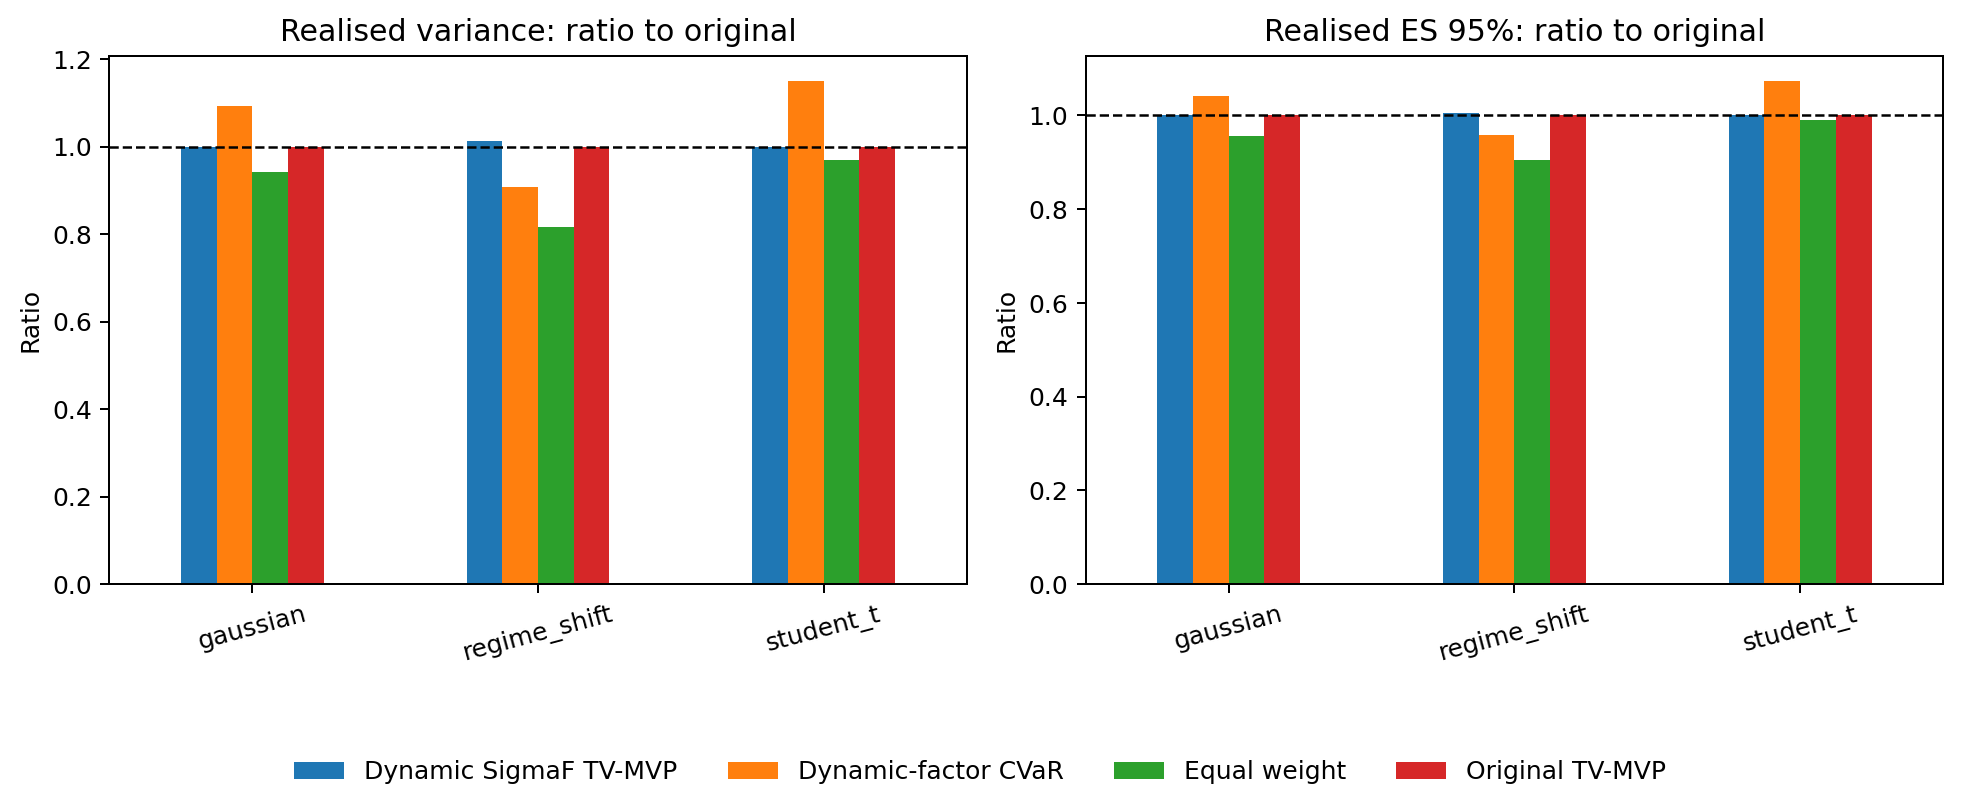
\includegraphics[width=0.94\textwidth]{simulation_stress_summary.png}
\caption{Mean realised variance and ES ratios to original TV-MVP. Values below one favour the displayed method, subject to the constraint caveat.}
\label{fig:simulation}
\end{figure}

\section{Robustness and sensitivity}

The robustness grid varies one parameter at a time from the common baseline and evaluates 1,399 post-2021 observations:
\begin{itemize}
  \item EWMA decay: 0.90, 0.94, 0.97;
  \item rolling window: 378, 504, 756 trading days;
  \item factor number: 2, 3, 5;
  \item CVaR confidence: 0.90, 0.95, 0.99;
  \item transaction cost: 0, 10, 25 basis points.
\end{itemize}

C-minus-B Sharpe difference remains negative across every EWMA decay (-0.0339 to -0.0187), window (-0.0461 to -0.0209), and factor count (-0.0422 to -0.0290). C-minus-B net return is also negative throughout. Baseline D-minus-B Sharpe varies substantially with confidence: -0.0154 at 90\%, -0.1332 at 95\%, and -0.0049 at 99\%. D-minus-B ES changes sign at 99\%. This instability is a sensitivity failure, not evidence for selecting 99\% after seeing the outcome.

Transaction costs monotonically worsen the dynamic model's net-return difference because turnover is high. The transaction-cost sweep recomputes net returns from fixed gross returns and turnover; it does not refit weights.

\begin{figure}[H]
\centering
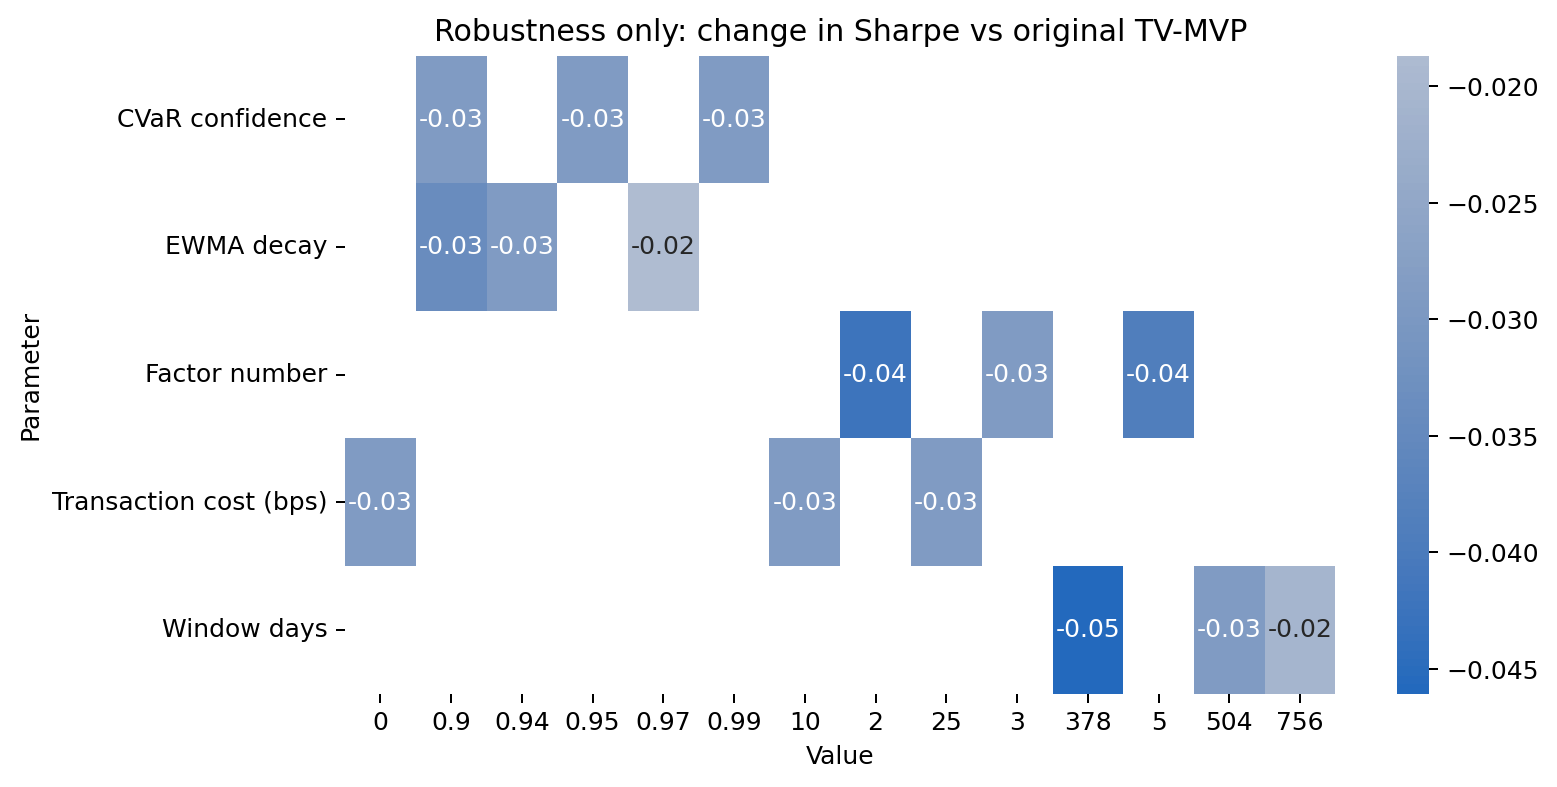
\includegraphics[width=0.88\textwidth]{sensitivity_heatmap.png}
\caption{Compact robustness heatmap. It shows dynamic-minus-original Sharpe only; CVaR sensitivity remains available in the CSV table.}
\label{fig:sensitivity}
\end{figure}

\section{Software implementation in detail}

\subsection{Module-to-method map}

\begin{longtable}{@{}p{0.28\textwidth}p{0.67\textwidth}@{}}
\caption{Python implementation map}\label{tab:module-map}\\
\toprule
File & Responsibility \\
\midrule
\endfirsthead
\toprule
File & Responsibility \\
\midrule
\endhead
\path{config.py} & YAML loading, required-section validation, and deep-copy dotted overrides. \\
\path{data.py} & Author MAT loading; Yahoo cache/download; completeness filter; adjusted-close returns; monthly endpoint positions; SHA-256 data hashes. \\
\path{factor.py} & Rule-of-thumb bandwidth, discrete Epanechnikov weights, local SVD/PCA at every date, least-squares scores and residuals, factor count approximation, principal angles. \\
\path{covariance.py} & Sparse residual correlation thresholding, ordinary and EWMA factor covariance, positive-definite eigenvalue repair. \\
\path{optimisation.py} & Equal weights, unconstrained/constrained MVP, empirical CVaR LP, filtered scenario generator, and regularised CVaR LP. \\
\path{backtest.py} & Shared rolling engine, matched/improved strategy modes, holdings drift, costs, covariance losses, diagnostics, scenario calibration, and ex-ante regimes. \\
\path{metrics.py} & Geometric return, volatility, Sharpe, maximum drawdown, empirical ES, monthly compounding, rolling ES, regime tables. \\
\path{inference.py} & Circular moving-block indices, all-pair intervals, primary-only p-values, original dynamic-regime test, and improved CVaR regime interaction. \\
\path{reproduction.py} & NumPy author DGP, supplied example workflow, reproduction tables and plots. \\
\path{empirical.py} & Core empirical orchestration, output writing, plots, and one-at-a-time sensitivity. \\
\path{fair_comparison.py} & Constraint-matched performance, monthly inference, calibration, yearly results, and cumulative plots. \\
\path{cvar_diagnostics.py} & Post-2021 mechanism analysis: calibration, concentration, allocation, factor shift, yearly performance, exploratory block intervals. \\
\path{improved_cvar.py} & Filtered/stressed/regularised ablation, primary inference, regime interaction, calibration, concentration, and corrected shared-legend plot. \\
\path{simulation.py} & Three DGPs, parallel replication, known-covariance error, Monte Carlo intervals, beat probabilities. \\
\path{plotting.py} & Core cumulative, rolling-risk, weights/turnover, factor, QQ, and sensitivity graphics. \\
\path{manifest.py} & Run time, platform, Git commit, seed, config hash, and package versions. \\
\bottomrule
\end{longtable}

\subsection{Numerical solvers}

Unconstrained MVP uses \code{numpy.linalg.solve}; matched MVP uses SciPy SLSQP with analytic gradient $2\Sigma w$, equality constraint, and box bounds. CVaR and regularised CVaR use \code{scipy.optimize.linprog(method="highs")} with explicit slack variables. All successful targets are checked indirectly in tests and output audits. In the final improved output, weight sums deviate from one by at most $2.21\times10^{-11}$, minimum weight is zero, and maximum weight is exactly 0.10.

\subsection{Randomness and reproducibility}

Project seed is 20260906. At empirical rebalance number $j$, baseline scenarios use seed $20260906+j$ and improved scenarios use $20260906+50000+j$. Bootstrap inference uses separately offset seeds. Simulations use offsets by DGP and replication. The manifest records Python 3.11.0 and package versions including NumPy 2.2.6, pandas 2.3.1, SciPy 1.16.0, Matplotlib 3.10.3, seaborn 0.13.2, PyYAML 6.0.3, and yfinance 0.2.65.

\subsection{Tests}

Seven tests currently pass:
\begin{enumerate}
  \item indefinite covariance matrices are repaired to positive definite;
  \item EWMA reacts to recent high variance;
  \item MVP and CVaR weights satisfy full-investment and cap constraints;
  \item filtered scenarios reproduce exactly under an identical seed, and regularised weights satisfy constraints;
  \item circular block indices are reproducible and contiguous within blocks;
  \item the regime classifier does not use the current return shock;
  \item changing future returns does not change earlier weights; matched optimisers also satisfy bounds and sums.
\end{enumerate}

The tests do not prove statistical correctness. Missing tests include equivalence to author MATLAB outputs under the same RNG, formal KKT residual checks for every optimisation, data-vendor revision detection, and end-to-end snapshot tests for every table.

\section{Limitations, threats to validity, and honest interpretation}

\subsection{Data validity}

\begin{itemize}
  \item Current constituents create survivorship bias and potentially favour stable winners.
  \item Yahoo adjusted-close histories can contain vendor adjustments and are not an institutional-quality point-in-time database.
  \item The sample covers one national equity market and one broad post-2015 period.
  \item Returns are not excess returns; the Sharpe-like measure assumes zero risk-free rate.
  \item Volume, spreads, borrow availability, corporate-action audit trails, taxes, and market impact are absent.
\end{itemize}

\subsection{Model validity}

\begin{itemize}
  \item The factor number is fixed at three empirically; factor-number uncertainty is not propagated.
  \item Local loading spaces can rotate sharply, and sign alignment cannot resolve general rotations within nearly tied eigenspaces.
  \item Residual covariance is treated as constant in B/C even though diagnostics motivate a dynamic alternative.
  \item The portable soft-threshold estimator is not the authors' \code{spcov} estimator.
  \item EWMA decay 0.94 implies only 32.33 effective observations and can be noisy.
  \item Empirical and filtered scenarios condition on estimated latent quantities without accounting for parameter uncertainty.
  \item Stress probability and multipliers are researcher-chosen rather than estimated from an independent training sample.
\end{itemize}

\subsection{Evaluation validity}

\begin{itemize}
  \item A one-month realised covariance is rank deficient when $p=39$ and contains substantial sampling noise.
  \item Daily ES annualisation by square-root-of-time is heuristic.
  \item Monthly ES is estimated from roughly 115 months in the full sample and only 68 post-2021 months; the 5\% tail is therefore extremely small.
  \item Moving blocks address short serial dependence but block length three is itself a modelling choice.
  \item The bootstrap p-value is an uncentred sign probability, not a null-imposed studentised test.
  \item Overlapping 504-day estimation windows make successive portfolios highly dependent even when realised monthly returns do not overlap.
  \item Many robustness configurations were examined. They are labelled exploratory, but researcher degrees of freedom remain.
  \item The improved model was motivated by observed baseline failure. Its existing NIFTY performance is not a clean holdout validation.
\end{itemize}

\subsection{Economic interpretation}

Equal weight has the strongest realised return and Sharpe. This may reflect a broad equal-weight premium, omitted estimation error, or survivorship-biased constituent selection; the project cannot identify causality. MVP portfolios achieve lower risk but sacrifice return. Raw CVaR is not inherently defective: it fails because its estimated tail distribution is a poor enough guide to the next month that optimisation overfits it. The filtered/regularised method improves the forecast inputs and controls the optimiser's freedom, but its apparent return advantage over matched MVP is statistically uncertain.

Backtest significance would not prove future profitability. Even a correctly sized historical test conditions on the market, assets, rules, costs, and structural regime that generated the sample. Deployment introduces model drift, liquidity feedback, strategy crowding, and unobserved implementation costs.

\section{Research programme for a publishable extension}

The repository supports a credible next-stage question:
\begin{quote}
Does conditionally scaled and regularised factor-based CVaR improve tail-risk portfolio selection relative to time-varying minimum variance, and under which data-generating regimes?
\end{quote}

A defensible confirmatory protocol should do the following before viewing new outcomes:

\begin{enumerate}
  \item Freeze D-FS and D-REG Version 1, including every multiplier and penalty.
  \item Designate primary estimands: realised monthly ES, tail-calibration score, turnover, and net return; choose a small number of directional hypotheses.
  \item Obtain point-in-time constituents and delisting returns for NIFTY and at least two independent markets.
  \item Use nested walk-forward tuning: at rebalance $t$, choose decay, stress, and regularisation only with data dated before $t$.
  \item Compare all strategies under both common matched constraints and a separate unconstrained/realistic mandate analysis.
  \item Add formal VaR coverage and independence diagnostics, ES forecast scoring, and conditional calibration tests.
  \item Add covariance forecast tests that respect noisy realised proxies, possibly with high-frequency realised covariance where available.
  \item Expand simulation axes: tail index, factor-strength, residual sparsity, loading smoothness, covariance break size, break timing, $p/T$, and transaction costs.
  \item Include the full improved-CVaR ablation in at least 100, preferably 500--1,000, matched-constraint replications per cell.
  \item Use a null-recentred or studentised dependent bootstrap and state a multiple-testing adjustment for the primary family.
  \item Preserve a genuinely untouched market or future period for final evaluation.
\end{enumerate}

The strongest defensible contribution is not ``CVaR beats MVP.'' It is that raw empirical CVaR is unusually sensitive to conditional-distribution and small-tail-sample error, while current-state filtering and portfolio regularisation can reduce calibration bias and optimiser instability. Whether this translates into robust economic superiority remains an open empirical question.

\section{Reproduction instructions}

From the repository root, using Python 3.10 or later:
\begin{lstlisting}
python3 -m pip install -e .
python3 scripts/run_all.py
\end{lstlisting}

Focused commands are:
\begin{lstlisting}
python3 scripts/run_reproduction.py
python3 scripts/run_empirical.py --with-sensitivity
python3 scripts/run_cvar_diagnostics.py
python3 scripts/run_fair_comparison.py
python3 scripts/run_improved_cvar.py
python3 scripts/run_simulations.py
\end{lstlisting}

The frozen data are used unless \code{--force-download} is explicitly supplied to a compatible entry point. Changing \path{project.seed} in \path{config.yaml} changes stochastic draws. The all-in-one run updates \path{results/run_manifest.json}. The improved empirical backtest is computationally heavier because each rebalance solves multiple LPs and performs factor/residual whitening.

\appendix

\section{Algorithmic pseudocode}

\subsection{Common rolling backtest}

\begin{lstlisting}
for each completed month-end t after 504 observations:
    estimation = returns[t-503 : t]
    holding    = returns[t+1 : next_month_end]

    fit local PCA at every date in estimation
    estimate score path and residual-vector path
    estimate sparse residual covariance
    estimate sample and EWMA factor covariance
    construct original and dynamic return covariance
    generate paired block-bootstrap scenarios

    solve targets for A, B, C, and D
    if matched/improved mode:
        impose identical long-only 10% cap on optimisers
    if improved mode:
        generate filtered/stressed scenarios
        solve filtered and regularised CVaR targets

    compute turnover from drifted previous holdings
    charge trading cost on first holding day
    realise portfolio using daily drifted weights
    evaluate forecast covariance against next-month proxy
    record factor, tail-calibration, and concentration diagnostics
\end{lstlisting}

\subsection{Moving-block inference}

\begin{lstlisting}
compound each strategy's net daily returns to calendar months
compute observed statistic for each strategy pair
for b = 1,...,1999:
    draw circular three-month blocks until sample length is reached
    apply identical month indices to both strategies
    recompute volatility, ES, and annualised net-return differences
report percentile 2.5% and 97.5% quantiles
report sign-probability p* only for registered pairs
\end{lstlisting}

\section{Complete configuration snapshot}

\begin{longtable}{@{}p{0.34\textwidth}p{0.58\textwidth}@{}}
\caption{Key configuration values}\label{tab:config}\\
\toprule
Parameter & Value \\
\midrule
\endfirsthead
\toprule
Parameter & Value \\
\midrule
\endhead
Seed; workers; annualisation & 20260906; 4; 252 \\
Data dates & 2015-01-01 to 2026-09-05 exclusive \\
Index & \code{\^NSEI} \\
Minimum history fraction & 0.985 \\
Rolling window; rebalance & 504 trading days; month-end \\
Factors; max reproduction factors & 3; 6 \\
Bandwidth & Rule of thumb, Equation \eqref{eq:bandwidth} \\
Residual threshold scale & 0.15 \\
Eigenvalue floor & $10^{-7}$ times covariance scale \\
Factor EWMA decay & 0.94 \\
Baseline CVaR & 95\%; 600 scenarios; 10-day blocks \\
Portfolio constraints & Long only; 10\% cap for CVaR and matched runs \\
Improved scenarios & 800; recent-start decay 0.995 \\
Improved residual covariance & EWMA decay 0.97; dynamic blend weight 0.50 \\
Stress mixture & 15\% probability; factor multiplier 1.50; residual multiplier 1.15 \\
Regularisation & Turnover 0.0010; equal-weight distance 0.00025 \\
Transaction costs & 10 bp per unit gross traded notional \\
Post-COVID start & 2021-01-01 \\
Rolling plotted risk & 63 days \\
High-volatility signal & 21-day index volatility; expanding 75th percentile; minimum 126 days; lagged \\
Bootstrap & 1,999 draws; three-month comparison blocks; 21-day regime blocks \\
Simulation & 100 replications; 20 assets; 180 training; 63 evaluation; two factors; Student-$t$ df 5; 350 scenarios \\
Sensitivity & $\lambda\in\{0.90,0.94,0.97\}$; $W\in\{378,504,756\}$; $K\in\{2,3,5\}$; CVaR $\in\{0.90,0.95,0.99\}$; costs $\in\{0,10,25\}$ bp \\
\bottomrule
\end{longtable}

\section{Result provenance}

Every major claim can be traced to a CSV rather than being read manually from a chart:

\begin{longtable}{@{}p{0.42\textwidth}p{0.51\textwidth}@{}}
\toprule
Evidence file & Content \\
\midrule
\endfirsthead
\toprule
Evidence file & Content \\
\midrule
\endhead
\path{reproduction_results.csv} & Manual target comparison and portable simulation metrics \\
\path{empirical_performance.csv} & Full-sample A--D gross/net performance \\
\path{pairwise_bootstrap_inference.csv} & All core pair intervals and primary-only p-values \\
\path{regime_performance.csv} & High/normal metrics from ex-ante index regime \\
\path{regime_benefit_test.csv} & Dynamic-covariance high-regime interaction \\
\path{covariance_forecast_summary.csv} & Frobenius and portfolio-risk loss summaries \\
\path{factor_diagnostics.csv} & Rebalance-by-rebalance factor evidence \\
\path{simulation_replications.csv} & All 1,200 strategy-replication rows across three DGPs \\
\path{simulation_summary.csv} & Mean, standard deviation, Monte Carlo interval \\
\path{simulation_beat_probabilities.csv} & Probability each method beats original TV-MVP \\
\path{sensitivity_summary.csv} & One-at-a-time robustness grid \\
\path{matched_post_covid_performance.csv} & Fair post-2021 comparison \\
\path{matched_post_covid_inference.csv} & Fair monthly bootstrap evidence \\
\path{matched_tail_calibration.csv} & Fitted and realised tail behaviour, concentration \\
\path{improved_cvar_post_covid_performance.csv} & Improved-CVaR ablation performance \\
\path{improved_cvar_post_covid_inference.csv} & Improved primary and exploratory intervals \\
\path{improved_cvar_tail_calibration.csv} & Scenario method, bias, exceedance, ranking, weights \\
\path{improved_cvar_regime_interaction.csv} & Improved high-minus-normal bootstrap \\
\bottomrule
\end{longtable}

\section{Glossary}

\begin{description}
  \item[Adjusted close] Vendor price adjusted for corporate actions such as splits and distributions.
  \item[Block bootstrap] Resampling consecutive observations rather than individual IID dates.
  \item[CVaR / expected shortfall] Mean loss in the tail beyond a specified confidence quantile.
  \item[Effective assets] Inverse Herfindahl concentration, $1/\sum_iw_i^2$.
  \item[EWMA] Exponentially weighted moving average, assigning larger weight to recent data.
  \item[Factor loading] Asset exposure to a latent common return shock.
  \item[Frobenius loss] Square root of the sum of squared matrix-entry forecast errors.
  \item[Local PCA] Principal components estimated with observations weighted by distance from a target date.
  \item[MVP] Fully invested portfolio minimising variance for a supplied covariance matrix.
  \item[Principal angle] Rotation-invariant measure of distance between factor-loading subspaces.
  \item[Scenario calibration gap] Realised holding-period CVaR minus fitted scenario CVaR.
  \item[Survivorship bias] Bias caused by constructing historical samples from securities known to survive to the present.
  \item[Turnover] One-half the $L_1$ difference between target and drifted pre-trade weights.
\end{description}

\clearpage
\begin{thebibliography}{99}

\bibitem{fan2024}
Q. Fan, R. Wu, Y. Yang, and W. Zhong,
``Time-varying minimum variance portfolio,''
\emph{Journal of Econometrics}, vol. 239, no. 2, article 105339, 2024.
\href{https://doi.org/10.1016/j.jeconom.2022.08.007}{doi:10.1016/j.jeconom.2022.08.007}.

\bibitem{fanmanual}
Q. Fan, R. Wu, Y. Yang, and W. Zhong,
\emph{Time-varying Minimum Variance Portfolio: A User's Manual}, 7 September 2022.
Supplied in this repository as \path{original_author_code/Manual.pdf}.

\bibitem{markowitz1952}
H. Markowitz,
``Portfolio selection,''
\emph{The Journal of Finance}, vol. 7, no. 1, pp. 77--91, 1952.
\href{https://doi.org/10.1111/j.1540-6261.1952.tb01525.x}{doi:10.1111/j.1540-6261.1952.tb01525.x}.

\bibitem{suwang2017}
L. Su and X. Wang,
``On time-varying factor models: Estimation and testing,''
\emph{Journal of Econometrics}, vol. 198, no. 1, pp. 84--101, 2017.
\href{https://doi.org/10.1016/j.jeconom.2016.12.004}{doi:10.1016/j.jeconom.2016.12.004}.

\bibitem{hongli2005}
Y. Hong and H. Li,
``Nonparametric specification testing for continuous-time models with applications to term structure of interest rates,''
\emph{The Review of Financial Studies}, vol. 18, no. 1, pp. 37--84, 2005.
\href{https://doi.org/10.1093/rfs/hhh006}{doi:10.1093/rfs/hhh006}.

\bibitem{baing2002}
J. Bai and S. Ng,
``Determining the number of factors in approximate factor models,''
\emph{Econometrica}, vol. 70, no. 1, pp. 191--221, 2002.
\href{https://doi.org/10.1111/1468-0262.00273}{doi:10.1111/1468-0262.00273}.

\bibitem{bientib2011}
J. Bien and R. J. Tibshirani,
``Sparse estimation of a covariance matrix,''
\emph{Biometrika}, vol. 98, no. 4, pp. 807--820, 2011.
\href{https://doi.org/10.1093/biomet/asr054}{doi:10.1093/biomet/asr054}.

\bibitem{rothman2012}
A. J. Rothman,
``Positive definite estimators of large covariance matrices,''
\emph{Biometrika}, vol. 99, no. 3, pp. 733--740, 2012.
\href{https://doi.org/10.1093/biomet/ass025}{doi:10.1093/biomet/ass025}.

\bibitem{rockafellar2000}
R. T. Rockafellar and S. Uryasev,
``Optimization of conditional value-at-risk,''
\emph{The Journal of Risk}, vol. 2, no. 3, 2000.
\href{https://doi.org/10.21314/JOR.2000.038}{doi:10.21314/JOR.2000.038}.

\bibitem{rockafellar2002}
R. T. Rockafellar and S. Uryasev,
``Conditional value-at-risk for general loss distributions,''
\emph{Journal of Banking and Finance}, vol. 26, no. 7, pp. 1443--1471, 2002.
\href{https://doi.org/10.1016/S0378-4266(02)00271-6}{doi:10.1016/S0378-4266(02)00271-6}.

\bibitem{acerbitasche2002}
C. Acerbi and D. Tasche,
``On the coherence of expected shortfall,''
\emph{Journal of Banking and Finance}, vol. 26, no. 7, pp. 1487--1503, 2002.
\href{https://doi.org/10.1016/S0378-4266(02)00283-2}{doi:10.1016/S0378-4266(02)00283-2}.

\bibitem{kunsch1989}
H. R. K\"unsch,
``The jackknife and the bootstrap for general stationary observations,''
\emph{The Annals of Statistics}, vol. 17, no. 3, pp. 1217--1241, 1989.
\href{https://doi.org/10.1214/aos/1176347265}{doi:10.1214/aos/1176347265}.

\end{thebibliography}

\end{document}
